\documentclass[a4paper]{article}
\usepackage[portuguese, english]{babel}
\usepackage{eso-pic} % marca de água para logos
\usepackage{fancyhdr}% logo para cabecalhos
\usepackage[a4paper,left=3cm,right=2cm,top=2.5cm,bottom=2.5cm, headheight=0.6in]{geometry}
\usepackage{palatino}
\usepackage[colorlinks=true,linkcolor=blue,citecolor=blue]{hyperref}
\usepackage{graphicx}
\usepackage{caption}
\usepackage{url}
\usepackage{subcaption}
\usepackage[utf8]{inputenc}
\usepackage[T1]{fontenc}
%% ODER: format ==         = "\mathrel{==}"
%% ODER: format /=         = "\neq "
%
%
\makeatletter
\@ifundefined{lhs2tex.lhs2tex.sty.read}%
  {\@namedef{lhs2tex.lhs2tex.sty.read}{}%
   \newcommand\SkipToFmtEnd{}%
   \newcommand\EndFmtInput{}%
   \long\def\SkipToFmtEnd#1\EndFmtInput{}%
  }\SkipToFmtEnd

\newcommand\ReadOnlyOnce[1]{\@ifundefined{#1}{\@namedef{#1}{}}\SkipToFmtEnd}
\usepackage{amstext}
\usepackage{amssymb}
\usepackage{stmaryrd}
\DeclareFontFamily{OT1}{cmtex}{}
\DeclareFontShape{OT1}{cmtex}{m}{n}
  {<5><6><7><8>cmtex8
   <9>cmtex9
   <10><10.95><12><14.4><17.28><20.74><24.88>cmtex10}{}
\DeclareFontShape{OT1}{cmtex}{m}{it}
  {<-> ssub * cmtt/m/it}{}
\newcommand{\texfamily}{\fontfamily{cmtex}\selectfont}
\DeclareFontShape{OT1}{cmtt}{bx}{n}
  {<5><6><7><8>cmtt8
   <9>cmbtt9
   <10><10.95><12><14.4><17.28><20.74><24.88>cmbtt10}{}
\DeclareFontShape{OT1}{cmtex}{bx}{n}
  {<-> ssub * cmtt/bx/n}{}
\newcommand{\tex}[1]{\text{\texfamily#1}}	% NEU

\newcommand{\Sp}{\hskip.33334em\relax}


\newcommand{\Conid}[1]{\mathit{#1}}
\newcommand{\Varid}[1]{\mathit{#1}}
\newcommand{\anonymous}{\kern0.06em \vbox{\hrule\@width.5em}}
\newcommand{\plus}{\mathbin{+\!\!\!+}}
\newcommand{\bind}{\mathbin{>\!\!\!>\mkern-6.7mu=}}
\newcommand{\rbind}{\mathbin{=\mkern-6.7mu<\!\!\!<}}% suggested by Neil Mitchell
\newcommand{\sequ}{\mathbin{>\!\!\!>}}
\renewcommand{\leq}{\leqslant}
\renewcommand{\geq}{\geqslant}
\usepackage{polytable}

%mathindent has to be defined
\@ifundefined{mathindent}%
  {\newdimen\mathindent\mathindent\leftmargini}%
  {}%

\def\resethooks{%
  \global\let\SaveRestoreHook\empty
  \global\let\ColumnHook\empty}
\newcommand*{\savecolumns}[1][default]%
  {\g@addto@macro\SaveRestoreHook{\savecolumns[#1]}}
\newcommand*{\restorecolumns}[1][default]%
  {\g@addto@macro\SaveRestoreHook{\restorecolumns[#1]}}
\newcommand*{\aligncolumn}[2]%
  {\g@addto@macro\ColumnHook{\column{#1}{#2}}}

\resethooks

\newcommand{\onelinecommentchars}{\quad-{}- }
\newcommand{\commentbeginchars}{\enskip\{-}
\newcommand{\commentendchars}{-\}\enskip}

\newcommand{\visiblecomments}{%
  \let\onelinecomment=\onelinecommentchars
  \let\commentbegin=\commentbeginchars
  \let\commentend=\commentendchars}

\newcommand{\invisiblecomments}{%
  \let\onelinecomment=\empty
  \let\commentbegin=\empty
  \let\commentend=\empty}

\visiblecomments

\newlength{\blanklineskip}
\setlength{\blanklineskip}{0.66084ex}

\newcommand{\hsindent}[1]{\quad}% default is fixed indentation
\let\hspre\empty
\let\hspost\empty
\newcommand{\NB}{\textbf{NB}}
\newcommand{\Todo}[1]{$\langle$\textbf{To do:}~#1$\rangle$}

\EndFmtInput
\makeatother
%
%
%
%
%
%
% This package provides two environments suitable to take the place
% of hscode, called "plainhscode" and "arrayhscode". 
%
% The plain environment surrounds each code block by vertical space,
% and it uses \abovedisplayskip and \belowdisplayskip to get spacing
% similar to formulas. Note that if these dimensions are changed,
% the spacing around displayed math formulas changes as well.
% All code is indented using \leftskip.
%
% Changed 19.08.2004 to reflect changes in colorcode. Should work with
% CodeGroup.sty.
%
\ReadOnlyOnce{polycode.fmt}%
\makeatletter

\newcommand{\hsnewpar}[1]%
  {{\parskip=0pt\parindent=0pt\par\vskip #1\noindent}}

% can be used, for instance, to redefine the code size, by setting the
% command to \small or something alike
\newcommand{\hscodestyle}{}

% The command \sethscode can be used to switch the code formatting
% behaviour by mapping the hscode environment in the subst directive
% to a new LaTeX environment.

\newcommand{\sethscode}[1]%
  {\expandafter\let\expandafter\hscode\csname #1\endcsname
   \expandafter\let\expandafter\endhscode\csname end#1\endcsname}

% "compatibility" mode restores the non-polycode.fmt layout.

\newenvironment{compathscode}%
  {\par\noindent
   \advance\leftskip\mathindent
   \hscodestyle
   \let\\=\@normalcr
   \let\hspre\(\let\hspost\)%
   \pboxed}%
  {\endpboxed\)%
   \par\noindent
   \ignorespacesafterend}

\newcommand{\compaths}{\sethscode{compathscode}}

% "plain" mode is the proposed default.
% It should now work with \centering.
% This required some changes. The old version
% is still available for reference as oldplainhscode.

\newenvironment{plainhscode}%
  {\hsnewpar\abovedisplayskip
   \advance\leftskip\mathindent
   \hscodestyle
   \let\hspre\(\let\hspost\)%
   \pboxed}%
  {\endpboxed%
   \hsnewpar\belowdisplayskip
   \ignorespacesafterend}

\newenvironment{oldplainhscode}%
  {\hsnewpar\abovedisplayskip
   \advance\leftskip\mathindent
   \hscodestyle
   \let\\=\@normalcr
   \(\pboxed}%
  {\endpboxed\)%
   \hsnewpar\belowdisplayskip
   \ignorespacesafterend}

% Here, we make plainhscode the default environment.

\newcommand{\plainhs}{\sethscode{plainhscode}}
\newcommand{\oldplainhs}{\sethscode{oldplainhscode}}
\plainhs

% The arrayhscode is like plain, but makes use of polytable's
% parray environment which disallows page breaks in code blocks.

\newenvironment{arrayhscode}%
  {\hsnewpar\abovedisplayskip
   \advance\leftskip\mathindent
   \hscodestyle
   \let\\=\@normalcr
   \(\parray}%
  {\endparray\)%
   \hsnewpar\belowdisplayskip
   \ignorespacesafterend}

\newcommand{\arrayhs}{\sethscode{arrayhscode}}

% The mathhscode environment also makes use of polytable's parray 
% environment. It is supposed to be used only inside math mode 
% (I used it to typeset the type rules in my thesis).

\newenvironment{mathhscode}%
  {\parray}{\endparray}

\newcommand{\mathhs}{\sethscode{mathhscode}}

% texths is similar to mathhs, but works in text mode.

\newenvironment{texthscode}%
  {\(\parray}{\endparray\)}

\newcommand{\texths}{\sethscode{texthscode}}

% The framed environment places code in a framed box.

\def\codeframewidth{\arrayrulewidth}
\RequirePackage{calc}

\newenvironment{framedhscode}%
  {\parskip=\abovedisplayskip\par\noindent
   \hscodestyle
   \arrayrulewidth=\codeframewidth
   \tabular{@{}|p{\linewidth-2\arraycolsep-2\arrayrulewidth-2pt}|@{}}%
   \hline\framedhslinecorrect\\{-1.5ex}%
   \let\endoflinesave=\\
   \let\\=\@normalcr
   \(\pboxed}%
  {\endpboxed\)%
   \framedhslinecorrect\endoflinesave{.5ex}\hline
   \endtabular
   \parskip=\belowdisplayskip\par\noindent
   \ignorespacesafterend}

\newcommand{\framedhslinecorrect}[2]%
  {#1[#2]}

\newcommand{\framedhs}{\sethscode{framedhscode}}

% The inlinehscode environment is an experimental environment
% that can be used to typeset displayed code inline.

\newenvironment{inlinehscode}%
  {\(\def\column##1##2{}%
   \let\>\undefined\let\<\undefined\let\\\undefined
   \newcommand\>[1][]{}\newcommand\<[1][]{}\newcommand\\[1][]{}%
   \def\fromto##1##2##3{##3}%
   \def\nextline{}}{\) }%

\newcommand{\inlinehs}{\sethscode{inlinehscode}}

% The joincode environment is a separate environment that
% can be used to surround and thereby connect multiple code
% blocks.

\newenvironment{joincode}%
  {\let\orighscode=\hscode
   \let\origendhscode=\endhscode
   \def\endhscode{\def\hscode{\endgroup\def\@currenvir{hscode}\\}\begingroup}
   %\let\SaveRestoreHook=\empty
   %\let\ColumnHook=\empty
   %\let\resethooks=\empty
   \orighscode\def\hscode{\endgroup\def\@currenvir{hscode}}}%
  {\origendhscode
   \global\let\hscode=\orighscode
   \global\let\endhscode=\origendhscode}%

\makeatother
\EndFmtInput
%
%================= lhs2tex=====================================================%
% -- desactivados:
%%format (uncurry (f)) = "\uncurry{" f "}"
%%format Either a b = a "+" b
%================= Standard packages ==========================================%
\usepackage[portuguese]{babel}
\usepackage[utf8]{inputenc}
%----------------- Date -------------------------------------------------------%
\def\mydate{
\ifcase\month\or
 Janeiro\or Fevereiro\or Março\or Abril\or Maio\or Junho\or Julho\or Agosto\or Setembro\or Outubro\or Novembro\or Dezembro\fi \ de \number\year
}
%----------------- verbatim ---------------------------------------------------%
\usepackage{fancyvrb}
%----------------- Using xy ---------------------------------------------------%
\usepackage[all]{xy}
\def\larrow#1#2#3{\xymatrix{ #3 & #1 \ar[l]_-{#2} }}
\def\rarrow#1#2#3{\xymatrix{ #1 \ar[r]^-{#2} & #3 }}
\def\u{u}                  % unidade de um mónade
\def\fun#1{{\sf #1}\index{Functor}}
%----------------- Using makeidx ----------------------------------------------%
\usepackage{makeidx}
\def\Bibtex{\href{http://www.bibtex.org/}{Bib\TeX}\index{Utilitário!LaTeX!\texttt{bibtex}}}
\def\Makeindex{\href{http://www.tex.ac.uk/ctan/indexing/makeindex/doc/makeindex.pdf}{\texttt{makeindex}}\index{Utilitário!LaTeX!\texttt{makeindex}}}
\def\GHCi{\ghci{GHCi}}
\def\ghci#1{\href{https://downloads.haskell.org/~ghc/latest/docs/html/users_guide/ghci.html}{#1}\index{Haskell!interpretador!GHCi}}
\def\IO{IO\index{Mónade!\texttt{IO}}}
\def\Latex{\LaTeX\index{\LaTeX}}
\def\LhsToTeX{\lhstotex{lhs2tex}}
\def\N{I\!\!N\index{Números naturais ($I\!\!N$)}}
\def\R{I\!\!R\index{Números reais ($I\!\!R$)}}
\def\Probability{\href{http://wiki.di.uminho.pt/twiki/bin/view/Education/CP/MaterialPedagogico}{Probability}\index{Haskell!Biblioteca!Probability}}
\def\TUG{TUG\index{TeX!TeX Users Group (TUG)}}
\def\alt#1#2{\mathopen{[}#1 , #2\mathclose{]}\index{Combinador ``pointfree''!\emph{either}}}	% "either" is reserved....
\def\ap#1#2{#1\,#2}
\def\bang{{!}\index{Função!\emph{bang}}}
\def\cata#1{\mathopen{(\!\ensuremath{\mskip1.5mu\}\mathbin{\#}\mathrm{1}\lambda \Varid{mathclose}\;\{\mskip1.5mu }\!)}\index{Combinador ``pointfree''!\emph{cata}}}
\def\dium{\htmladdnormallink{Departamento de Informática}{http://www.di.uminho.pt/}\index{U.Minho!Departamento de Informática}}
\def\file#1{\texttt{#1}\index{Ficheiro!\texttt{#1}}}
\def\haskell#1{\href{http://www.haskell.org}{#1}\index{Haskell}}
\def\litp#1{\href{http://www.literateprogramming.com}{#1}\index{Programação literária}}
\def\lhstotex#1{\href{https://hackage.haskell.org/package/lhs2tex}{#1}\index{Haskell!``Literate Haskell''!lhs2TeX}}
\def\LTree{\href{http://wiki.di.uminho.pt/twiki/pub/Education/CP1314/MaterialPedagogico/LTree.hs}{LTree}\index{Cálculo de Programas!Material Pedagógico!LTree.hs}}
\def\List{\href{http://wiki.di.uminho.pt/twiki/pub/Education/CP1314/MaterialPedagogico/List.hs}{List}\index{Cálculo de Programas!Material Pedagógico!List.hs}}
\def\ControlParallelStrategies{\href{https://hackage.haskell.org/package/parallel-3.1.0.1/docs/Control-Parallel-Strategies.html}{Control.Parallel.Strategies}\index{Haskell!Control!Parallel.Strategies}}
\def\PFP{\href{http://web.engr.oregonstate.edu/~erwig/pfp}{PHP}\index{Haskell!Biblioteca!PFP}}
\def\XFreedom{\href{http://www.x3dom.org}{X3DOM}\index{Utilitário!X3DOM}}
\def\BTree{\href{http://wiki.di.uminho.pt/twiki/pub/Education/CP1314/MaterialPedagogico/BTree.hs}{BTree}\index{Cálculo de Programas!Material Pedagógico!BTree.hs}}
\def\material#1{\href{http://wiki.di.uminho.pt/twiki/bin/view/Education/CP/MaterialPedagogico}{#1}\index{Cálculo de Programas!Material Pedagógico}}
\def\cp#1{\href{http://wiki.di.uminho.pt/twiki/bin/view/Education/CP/WebHome}{#1}\index{Cálculo de Programas}}
\def\MaterialPedagogico{\material{material pedagógico}}
\def\haskellf#1{\texttt{#1}\index{Função!\texttt{#1}}}
\def\fractal{\href{http://pt.wikipedia.org/wiki/Fractal}{fractal}\index{Fractal}}
\def\sierp#1{\href{http://en.wikipedia.org/wiki/Sierpinski_triangle}{#1}\index{Fractal!Tri\^angulo de Sierpinski}}
\def\psierp#1{\href{http://en.wikipedia.org/wiki/Sierpinski_triangle}{#1}\index{Fractal!Pirâmide de Sierpinski}}
\def\hcata{cata\index{Combinador ``pointfree''!\emph{cata}}}
\def\iso{\mathbin{\cong}\index{Relação de isomorfismo}}
\def\kons#1{\underline{#1}\index{Combinador ``pointfree''!função constante}}
\def\lhaskell#1{#1\index{Haskell!``Literate Haskell''}}
\def\mutu#1#2{\mathopen{\lhd}#1 , #2\mathclose{\rhd}\index{Combinador ``pointfree''!\emph{mutu}}}
\def\obrigatorio{${}^\dagger\ $\index{Exercícios obrigatórios}}
\def\p#1{\pi_{#1}\index{Função!$\pi_#1$}}
\def\sana#1{\mathopen{[\!(}#1\mathclose{)\!]}\index{Combinador ``pointfree''!\emph{ana}}}
\def\spara#1{\mathopen{\langle\![}#1\mathclose{]\!\rangle}\index{Combinador ``pointfree''!\emph{para}}}
\def\split#1#2{\mathopen{\langle}#1 , #2\mathclose{\rangle}\index{Combinador ``pointfree''!\emph{split}}} % <a,b,...z>
\def\texcmd#1{\texttt{#1}\index{\LaTeX!macro!\texttt{#1}}}
\def\trans#1{\overline{#1\rule{0pt}{.6em}}\index{Combinador ``pointfree''!transposição}}
\def\uncurry #1{\widehat{#1}\index{Função!\emph{uncurry}}}
\def\xypic#1{\textsc{#1}\index{\LaTeX!pacote!XY-pic}}
%----------------- Extracted from jnobasics.sty -------------------------------%
\long\def\pdfout#1{\relax}
\def\mcond#1#2#3{#1 \rightarrow #2 , #3}
\newenvironment{lcbr}{\left\{\begin{array}{l}}{\end{array}\right.}
\newenvironment{calculation}{\begin{eqnarray*}&&}{\end{eqnarray*}}
\def\eg{\emph{eg.}}
\def\esimo#1{#1${.\kern-.1em}^{\super{o}}$}
\def\esima#1{#1${.\kern-.1em}^{\super{a}}$}
\def\super#1{\mbox{{\scriptsize #1}}}
\def\traco{\noindent\mbox{}\hrulefill\mbox{} \\*}
\def\law#1#2#3#4{%
        \makebox[.25\textwidth][l]{\textbf{#2}}
&&
        \begin{array}{rcl}#4\end{array}
        \label{eq:#1}
%	\index{Lei!#2}
}
\def\comp{\mathbin{\cdot}}
\def\implied{\mathbin\Leftarrow}
\def\deff{\stackrel{\rm def}{=}}          % Function definition symbol
\def\just#1#2{\\ &#1& \rule{2em}{0pt} \{ \mbox{\rule[-.7em]{0pt}{1.8em} \small #2 \/} \} \nonumber\\ && }
\def\kcomp{\mathbin{\bullet}}
%----------------- Importing/modifying isolatin1 ------------------------------%
%\usepackage{isolatin1}
%\catcode181=13  \def^^b5{\mu}				% 181, '265, "b5
%\@ifundefined{lguill}{\def^^ab{``}}{\def^^ab{\lguill}}
%\@ifundefined{rguill}{\def^^bb{''}}{\def^^bb{\rguill}}
%\catcode186=13  \def^^ba{${\kern-.1em}^{\mbox{\scriptsize o}}$}      % 186, '272, "ba
%\catcode183=13  \def^^b7{\comp}     % 183, '267, "b7
%----------------- Exercise format --------------------------------------------%
\newcounter{exercise}
\def\theexercise{\arabic{exercise}}
%
\newenvironment{exercise}%
{\refstepcounter{exercise}
     \setlength{\parindent}{1em}
%    \setlength{\parskip}{\baselineskip}
%    \medskip
     \noindent
     {\bf Exercício~\theexercise.}
\addcontentsline{loe}{subsection}{\numberline{}{{\rm \hskip-6em Exercise \arabic{exercise}}}}}%
{~\\~\\ \traco \bigskip} %\hrule\bigskip}
%----------------- WWW interfacing desabled -----------------------------------%
\let\pisca=\relax
\def\quoteId#1#2{\textsl{#1}}
\def\quoteUrl#1#2{\texttt{#2}}
\let\htmladdnormallink=\quoteId             % HTML links disabled by default
%----------------- Shortcuts --------------------------------------------------%
\def\Haskell{\haskell{Haskell}}
\def\bb#1#2{{\fun B}(#1,#2)}
\def\b{\fun B}
\def\ff#1{\ap\f{#1}}
\def\fff#1{\ap{\f^2}{#1}}
\def\f{\fun F}
\def\gg#1{\ap\g{#1}}
\def\g{\fun G}
\def\muF{\mu\fun F}
\def\tf#1{\ap{\fun T}#1}
%----------------- testing ----------------------------------------------------%
\newtheorem{teste}{\underline{Testes unitários}}
%----------------- fim ----- ----------------------------------------------------%

%------------------- Comandos ---------------------%
%\renewcommand{\headheight}{0.6in}
\setlength{\headwidth}{\textwidth}
\fancyhead[L]{}% empty left
\fancyhead[L]{ % right
   
\includegraphics[height=0.53in]{logo-ee.jpg} % LOGO Cabeçalhho
}
\pagestyle{fancy}

\setlength{\unitlength}{1mm}
\newcommand\BackgroundPic[3]{
\put(#2,#3){\parbox[b][\paperheight]{\paperwidth}{
\vfill
\centering
\includegraphics{#1}
\vfill
}}}

\title{
		    Cálculo de Programas
\\
		Trabalho Prático
\\
		LCC+LEI --- Ano Lectivo de 2014/15
}

\author{
		 
\includegraphics{dium.jpg}
\\
		Departamento de Informática - Universidade do Minho
}

%\newcommand{\at}{\makeatletter @ \makeatother}

\date\mydate
\makeindex
\begin{document}
%--- Logo Capa ---%
\AddToShipoutPicture*{\BackgroundPic{logo_eeng}{-210}{370}} % LOGO CAPA
\maketitle

\vspace{40pt}
%\begin{figure}[h]
%\section{Grupo}
 \huge Grupo\\ \vspace{10pt}
	\vspace{10pt}
	\begin{figure}[h]
	%	\hspace{20pt}
	        \begin{subfigure}[b]{0.30\textwidth}
	                \centering
	                \includegraphics[width=\textwidth]{carlos.jpg}
		       \caption{nome : Carlos Gonçalves \\
				    número : xxxxxxx \\
				    mail :  xxxxxxxx.xxx  \\}
	                %\label{fig:carlos}
	        \end{subfigure}
		\hfill
		 \begin{subfigure}[b]{0.30\textwidth}
	                \centering
	                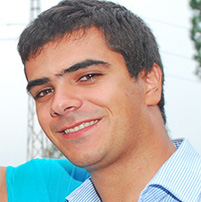
\includegraphics[width=\textwidth]{joao.jpg}
		       \caption{nome : João Rua \\
				    número : 41841 \\
				    mail : joaorua at mail.com \\}
	                %\label{fig:joao}
	        \end{subfigure}
		\hfill
		  \begin{subfigure}[b]{0.30\textwidth}
	                \centering
	                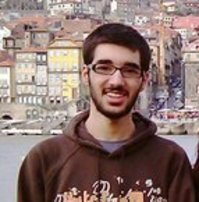
\includegraphics[width=\textwidth]{miguel.jpg}
		       \caption{nome : Miguel Guimarães \\
				    número : 66822 \\
				    mail :  migueguimaraess at hotmail.com  \\}
	                %\label{fig:miguel}
	        \end{subfigure}
		\hfill
	\end{figure}
%\end{figure}
\large
\newpage
\tableofcontents

\newpage

\section{Preâmbulo}

A disciplina de Cálculo de Programas tem como objectivo principal ensinar
a programação de computadores como uma disciplina científica. Para isso
parte-se de um repertório de \emph{combinadores} que formam uma álgebra da
programação (conjunto de leis universais e seus corolários) e usa-se esses
combinadores para construir programas \emph{composicionalmente}, isto é,
compondo programas já existentes.
  
Na sequência pedagógica dos planos de estudo dos dois cursos que têm esta disciplina,
restringe-se a aplicação deste método ao desenvolvimento de programas funcionais na linguagem \Haskell.

O presente trabalho tem por objectivo concretizar na prática os objectivos
da disciplina, colocando os alunos perante problemas de programação que
deverão ser abordados composicionalmente e implementados em \Haskell.
Há ainda um outro objectivo: o de ensinar a documentar programas e
a produzir textos técnico-científicos de qualidade.

\section{Documentação}
Para cumprir de forma integrada e simples os objectivos enunciados acima
vamos recorrer a uma técnica de programa\-ção dita \litp{literária} \cite{Kn92},
cujo princípio base é o seguinte:
\begin{quote}\em
Um programa e a sua documentação devem coincidir.
\end{quote}
Por outras palavras, o código fonte e a sua documentação deverão constar
do mesmo documento (ficheiro).

O ficheiro \texttt{cp1415t.pdf} que está a ler é já um exemplo de \litp{programação
literária}: foi gerado a partir do texto fonte \texttt{cp1415t.lhs}\footnote{O
suffixo `lhs' quer dizer \emph{\lhaskell{literate Haskell}}.} que encontrará
no \MaterialPedagogico\ desta disciplina descompactando o ficheiro \texttt{cp1415t.zip}
e executando
\begin{Verbatim}[fontsize=\small]
    lhs2TeX cp1415t.lhs > cp1415t.tex
    pdflatex cp1415t
\end{Verbatim}
em que \texttt\LhsToTeX\ é um pre-processador que faz ``pretty printing''
de código Haskell em \LaTeX\ e que deve desde já instalar a partir do endereço
\begin{quote}\tt\small
\lhstotex{https://hackage.haskell.org/package/lhs2tex}.
\end{quote}
Por outro lado, o mesmo ficheiro \texttt{cp1415t.lhs} é executável e contém
o ``kit'' básico, escrito em \Haskell, para realizar o trabalho. Basta executar
\begin{Verbatim}[fontsize=\small]
    ghci cp1415t.lhs
\end{Verbatim}
para ver que assim é: 
\begin{quote}
\begin{Verbatim}[fontsize=\small]
GHCi, version 7.8.3: http://www.haskell.org/ghc/  :? for help
Loading package ghc-prim ... linking ... done.
Loading package integer-gmp ... linking ... done.
Loading package base ... linking ... done.
[ 1 of 11] Compiling ListUtils        ( ListUtils.hs, interpreted )
[ 2 of 11] Compiling Cp               ( Cp.hs, interpreted )
[ 3 of 11] Compiling BTree            ( BTree.hs, interpreted )
[ 4 of 11] Compiling LTree            ( LTree.hs, interpreted )
[ 5 of 11] Compiling Exp              ( Exp.hs, interpreted )
[ 6 of 11] Compiling Nat              ( Nat.hs, interpreted )
[ 7 of 11] Compiling Show             ( Show.hs, interpreted )
[ 8 of 11] Compiling Probability      ( Probability.hs, interpreted )
[ 9 of 11] Compiling List             ( List.hs, interpreted )
[10 of 11] Compiling X3d              ( X3d.hs, interpreted )
[11 of 11] Compiling Main             ( cp1415t.lhs, interpreted )
Ok, modules loaded: List, Show, Nat, Exp, Cp, BTree, LTree, X3d,
Probability, Main, ListUtils.
\end{Verbatim}
\end{quote}
O facto de o interpretador carregar as bibliotecas do \MaterialPedagogico\ da disciplina,
entre outras, deve-se ao facto de, neste mesmo sítio do texto fonte,
se ter inserido o seguinte código \Haskell:

\begin{hscode}\SaveRestoreHook
\column{B}{@{}>{\hspre}l<{\hspost}@{}}%
\column{E}{@{}>{\hspre}l<{\hspost}@{}}%
\>[B]{}\mathbf{import}\;\Conid{\Conid{Data}.List}{}\<[E]%
\\
\>[B]{}\mathbf{import}\;\Conid{\Conid{System}.Process}{}\<[E]%
\\
\>[B]{}\mathbf{import}\;\Conid{Cp}{}\<[E]%
\\
\>[B]{}\mathbf{import}\;\Conid{List}{}\<[E]%
\\
\>[B]{}\mathbf{import}\;\Conid{Nat}{}\<[E]%
\\
\>[B]{}\mathbf{import}\;\Conid{Exp}{}\<[E]%
\\
\>[B]{}\mathbf{import}\;\Conid{BTree}{}\<[E]%
\\
\>[B]{}\mathbf{import}\;\Conid{LTree}{}\<[E]%
\\
\>[B]{}\mathbf{import}\;\Conid{X3d}{}\<[E]%
\\
\>[B]{}\mathbf{import}\;\Conid{\Conid{Control}.\Conid{Parallel}.Strategies}{}\<[E]%
\\
\>[B]{}\mathbf{import}\;\Conid{Probability}\;\Varid{hiding}\;(\mcond{\cdot }{\cdot }{\cdot }){}\<[E]%
\\
\>[B]{}\mathbf{import}\;\Conid{\Conid{System}.Environment}\;(\Varid{getArgs}){}\<[E]%
\ColumnHook
\end{hscode}\resethooks

\noindent Abra o ficheiro \texttt{cp1415t.lhs} no seu editor de texto preferido
e verifique que assim é: todo o texto que se encontra dentro do ambiente
\begin{quote}\small\tt
\text{\tt \char92{}begin\char123{}code\char125{}}
\\ ... \\
\text{\tt \char92{}end\char123{}code\char125{}}
\end{quote}
vai ser seleccionado pelo \GHCi\ para ser executado.

\section{Como realizar o trabalho}
Este trabalho teórico-prático deve ser realizado por grupos de três alunos.
Os detalhes da avaliação (datas para submissão do relatório e sua defesa
oral) são os que forem publicados na \cp{página da disciplina} na \emph{internet}.

Recomenda-se uma abordagem equilibrada e participativa dos membros do grupo
de trabalho por forma a poderem responder às questões que serão colocadas
na defesa oral do relatório.

Em que consiste, então, o \emph{relatório} a que se refere o parágrafo anterior?
É a edição do texto que está a ser lido, preenchendo o anexo \ref{sec:resolucao}
com as respostas. O relatório deverá conter ainda a identificação dos membros
do grupo de trabalho, na folha de rosto.

Para gerar o PDF integral do relatório deve-se ainda correr os comando seguintes,
que actualizam a bibliografia (com \Bibtex) e o índice remissivo (com \Makeindex)
\begin{Verbatim}[fontsize=\small]
    bibtex cp1415t.aux
    makeindex cp1415t.idx
\end{Verbatim}
e recompilar o texto como acima se indicou.

\section{Parte A}
Nesta primeira parte do trabalho pretende-se averiguar a capacidade de utilização
por parte dos alunos das bibliotecas fornecidas no \MaterialPedagogico\ da
disciplina. Algumas respostas são validadas por testes unitários. Sempre
que o resultado de um teste unitário for \ensuremath{\Conid{False}}, a solução proposta falha
a validação e deve ser revista.

\subsection{Biblioteca \LTree}\label{sec:LTree}
\begin{enumerate}
\item	A seguinte função
\begin{hscode}\SaveRestoreHook
\column{B}{@{}>{\hspre}l<{\hspost}@{}}%
\column{E}{@{}>{\hspre}l<{\hspost}@{}}%
\>[B]{}\Varid{balanced}\;(\Conid{Leaf}\;\anonymous )\mathrel{=}\Conid{True}{}\<[E]%
\\
\>[B]{}\Varid{balanced}\;(\Conid{Fork}\;(\Varid{t},\Varid{t'}))\mathrel{=}\Varid{balanced}\;\Varid{t}\mathrel{\wedge}\Varid{balanced}\;\Varid{t'}\mathrel{\wedge}\Varid{abs}\;(\Varid{depth}\;\Varid{t}\mathbin{-}\Varid{depth}\;\Varid{t'})\leq \mathrm{1}{}\<[E]%
\ColumnHook
\end{hscode}\resethooks
testa se uma árvore binária está equilibrada ou não. Defina como catamorfismo
em \LTree\ a função auxiliar \ensuremath{\Varid{depth}}.
\item Seja dada:
\begin{hscode}\SaveRestoreHook
\column{B}{@{}>{\hspre}l<{\hspost}@{}}%
\column{E}{@{}>{\hspre}l<{\hspost}@{}}%
\>[B]{}\Varid{t}\mathrel{=}\Conid{Fork}\;(\Conid{Fork}\;(\Conid{Leaf}\;\mathrm{10},\Conid{Fork}\;(\Conid{Leaf}\;\mathrm{2},\Conid{Fork}\;(\Conid{Leaf}\;\mathrm{5},\Conid{Leaf}\;\mathrm{3}))),\Conid{Leaf}\;\mathrm{23}){}\<[E]%
\ColumnHook
\end{hscode}\resethooks
\begin{teste}
Verifique que árvore \ensuremath{\Varid{t}} está desequilibrada:
\begin{hscode}\SaveRestoreHook
\column{B}{@{}>{\hspre}l<{\hspost}@{}}%
\column{E}{@{}>{\hspre}l<{\hspost}@{}}%
\>[B]{}\Varid{test01}\mathrel{=}\Varid{balanced}\;\Varid{t}\equiv \Conid{False}{}\<[E]%
\ColumnHook
\end{hscode}\resethooks
\end{teste}
\item Recorrendo a funções da biblioteca \LTree,
escreva numa única linha de Haskell a função
\begin{hscode}\SaveRestoreHook
\column{B}{@{}>{\hspre}l<{\hspost}@{}}%
\column{E}{@{}>{\hspre}l<{\hspost}@{}}%
\>[B]{}\Varid{balance}\mathbin{::}\Conid{LTree}\;\Varid{a}\to \Conid{LTree}\;\Varid{a}{}\<[E]%
\ColumnHook
\end{hscode}\resethooks
que equilibra uma qualquer árvore binária.
\begin{teste}
Verifique que \ensuremath{\Varid{balance}\;\Varid{t}} é uma árvore equilibrada:
\begin{hscode}\SaveRestoreHook
\column{B}{@{}>{\hspre}l<{\hspost}@{}}%
\column{E}{@{}>{\hspre}l<{\hspost}@{}}%
\>[B]{}\Varid{test02}\mathrel{=}\Varid{balanced}\;(\Varid{balance}\;\Varid{t})\equiv \Conid{True}{}\<[E]%
\ColumnHook
\end{hscode}\resethooks
\end{teste}
\end{enumerate}

\subsection{Biblioteca \BTree}\label{sec:BTree}
Pretende-se construir um anamorfismo que produza uma árvore binária de procura
\emph{equilibrada} que contenha o intervalo definido por dois inteiros \ensuremath{(\Varid{n},\Varid{m})}:
\begin{hscode}\SaveRestoreHook
\column{B}{@{}>{\hspre}l<{\hspost}@{}}%
\column{E}{@{}>{\hspre}l<{\hspost}@{}}%
\>[B]{}\Varid{abpe}\;(\Varid{n},\Varid{m})\mathrel{=}\Varid{anaBTree}\;\Varid{qsplit}\;(\Varid{n},\Varid{m}){}\<[E]%
\ColumnHook
\end{hscode}\resethooks
Comece por definir o gene \ensuremath{\Varid{qsplit}} e depois construa a árvore 
\begin{hscode}\SaveRestoreHook
\column{B}{@{}>{\hspre}l<{\hspost}@{}}%
\column{E}{@{}>{\hspre}l<{\hspost}@{}}%
\>[B]{}\Varid{t1}\mathrel{=}\Varid{abpe}\;(\mathrm{20},\mathrm{30}){}\<[E]%
\ColumnHook
\end{hscode}\resethooks
que será precisa na secção \ref{sec:parBTreeMap}.
\begin{teste}
Faça os testes seguintes:
\begin{hscode}\SaveRestoreHook
\column{B}{@{}>{\hspre}l<{\hspost}@{}}%
\column{E}{@{}>{\hspre}l<{\hspost}@{}}%
\>[B]{}\Varid{test03a}\mathrel{=}\Varid{qsplit}\;(\mathrm{4},\mathrm{30})\equiv i_2\;(\mathrm{17},((\mathrm{4},\mathrm{16}),(\mathrm{18},\mathrm{30}))){}\<[E]%
\\
\>[B]{}\Varid{test03b}\mathrel{=}\Varid{qsplit}\;(\mathrm{4},\mathrm{3})\equiv i_1\;(){}\<[E]%
\\
\>[B]{}\Varid{test03c}\mathrel{=}\Varid{qsplit}\;(\mathrm{0},\mathrm{0})\equiv i_1\;(){}\<[E]%
\\
\>[B]{}\Varid{test03d}\mathrel{=}\Varid{qsplit}\;(\mathrm{1},\mathrm{1})\equiv i_2\;(\mathrm{1},((\mathrm{1},\mathrm{0}),(\mathrm{2},\mathrm{1}))){}\<[E]%
\\
\>[B]{}\Varid{test03e}\mathrel{=}\Varid{balBTree}\;\Varid{t1}\equiv \Conid{True}{}\<[E]%
\\
\>[B]{}\Varid{test03f}\mathrel{=}\Varid{inordt}\;\Varid{t1}\equiv [\mskip1.5mu \mathrm{20}\mathinner{\ldotp\ldotp}\mathrm{30}\mskip1.5mu]{}\<[E]%
\ColumnHook
\end{hscode}\resethooks
\end{teste}

\subsection{Biblioteca para listas com sentinelas}\label{sec:SList}
Considere o tipo de dados que representa listas finitas com uma sentinela no fim:
\begin{hscode}\SaveRestoreHook
\column{B}{@{}>{\hspre}l<{\hspost}@{}}%
\column{E}{@{}>{\hspre}l<{\hspost}@{}}%
\>[B]{}\mathbf{data}\;\Conid{SList}\;\Varid{a}\;\Varid{b}\mathrel{=}\Conid{Sent}\;\Varid{b}\mid \Conid{Cons}\;(\Varid{a},\Conid{SList}\;\Varid{a}\;\Varid{b})\;\mathbf{deriving}\;(\Conid{Show},\Conid{Eq}){}\<[E]%
\ColumnHook
\end{hscode}\resethooks
\begin{enumerate}
\item	Derive os isomorfismos \ensuremath{\Varid{inSList}} e \ensuremath{\Varid{outSList}}, adicione-os a este ficheiro
e passe aos testes que se seguem.
\begin{teste}
Faça os testes seguintes:
\begin{hscode}\SaveRestoreHook
\column{B}{@{}>{\hspre}l<{\hspost}@{}}%
\column{E}{@{}>{\hspre}l<{\hspost}@{}}%
\>[B]{}\Varid{test04a}\mathrel{=}\mathbf{let}\;\Varid{x}\mathrel{=}\Conid{Cons}\;(\mathrm{1},\Conid{Sent}\;\text{\tt \char34 end\char34})\;\mathbf{in}\;\Varid{inSList}\;(\Varid{outSList}\;\Varid{x})\equiv \Varid{x}{}\<[E]%
\\
\>[B]{}\Varid{test04b}\mathrel{=}\mathbf{let}\;\Varid{x}\mathrel{=}i_2\;(\text{\tt \char34 ola\char34},\Conid{Sent}\;\text{\tt \char34 2\char34})\;\mathbf{in}\;\Varid{outSList}\;(\Varid{inSList}\;\Varid{x})\equiv \Varid{x}{}\<[E]%
\ColumnHook
\end{hscode}\resethooks
\end{teste}
\item Derive os combinadores \ensuremath{\Varid{cataSList}}, \ensuremath{\Varid{anaSList}} e \ensuremath{\Varid{hyloSList}},
e mostre que a função \ensuremath{\Varid{merge}} da biblioteca \LTree\ se pode escrever da forma seguinte,
\begin{hscode}\SaveRestoreHook
\column{B}{@{}>{\hspre}l<{\hspost}@{}}%
\column{E}{@{}>{\hspre}l<{\hspost}@{}}%
\>[B]{}\Varid{merge'}\mathbin{::}\Conid{Ord}\;\Varid{a}\Rightarrow ([\mskip1.5mu \Varid{a}\mskip1.5mu],[\mskip1.5mu \Varid{a}\mskip1.5mu])\to [\mskip1.5mu \Varid{a}\mskip1.5mu]{}\<[E]%
\\
\>[B]{}\Varid{merge'}\mathrel{=}\Varid{hyloSList}\;\alt{\Varid{id}}{\Varid{cons}}\;\Varid{mgen}{}\<[E]%
\ColumnHook
\end{hscode}\resethooks
para um dado gene \ensuremath{\Varid{mgen}} que deverá definir.
\begin{teste}
Faça os seguintes testes:
\begin{hscode}\SaveRestoreHook
\column{B}{@{}>{\hspre}l<{\hspost}@{}}%
\column{21}{@{}>{\hspre}l<{\hspost}@{}}%
\column{E}{@{}>{\hspre}l<{\hspost}@{}}%
\>[B]{}\Varid{test05a}\mathrel{=}\Varid{mgen}\;{}\<[21]%
\>[21]{}([\mskip1.5mu \mathrm{0},\mathrm{2},\mathrm{5}\mskip1.5mu],[\mskip1.5mu \mathrm{0},\mathrm{6}\mskip1.5mu])\equiv i_2\;(\mathrm{0},([\mskip1.5mu \mathrm{2},\mathrm{5}\mskip1.5mu],[\mskip1.5mu \mathrm{0},\mathrm{6}\mskip1.5mu])){}\<[E]%
\\
\>[B]{}\Varid{test05b}\mathrel{=}\Varid{mgen}\;([\mskip1.5mu \mathrm{0},\mathrm{2},\mathrm{5}\mskip1.5mu],[\mskip1.5mu \mskip1.5mu])\equiv i_1\;[\mskip1.5mu \mathrm{0},\mathrm{2},\mathrm{5}\mskip1.5mu]{}\<[E]%
\\
\>[B]{}\Varid{test05c}\mathrel{=}\Varid{merge'}\;([\mskip1.5mu \mskip1.5mu],[\mskip1.5mu \mathrm{0},\mathrm{6}\mskip1.5mu])\equiv [\mskip1.5mu \mathrm{0},\mathrm{6}\mskip1.5mu]{}\<[E]%
\ColumnHook
\end{hscode}\resethooks
\end{teste}
\end{enumerate}

\section{Parte B}
O \sierp{triângulo de Sierpinski} é uma figura \fractal\ que
tem o aspecto da figura \ref{fig:sierp1} e que se
obtém da seguinte forma: considere-se um triângulo rectângulo e
isósceles $A$ cujos catetos têm comprimento $s$. A estrutura \fractal\ é
criada desenhando-se três triângulos no interior de $A$, todos eles
rectângulos e isósceles e com catetos de comprimento $s/2$. Este passo
é depois repetido para cada um dos triângulos desenhados, e assim
sucessivamente. O resultado dos cinco primeiros passos é dado na
Fig.~\ref{fig:sierp1}.

\begin{figure}
\begin{center}
	
\includegraphics[width=0.4\textwidth]{media/sierp1.jpg}
\end{center}
	\caption{Um \sierp{triângulo de Sierpinski}}\label{fig:sierp1}
\end{figure}

Um \sierp{triângulo de Sierpinski} é gerado repetindo-se
infinitamente o processo acima descrito. No entanto, para efeitos de
visualização num monitor, cuja resolução é forçosamente finita,
faz sentido escolher uma representação adequada do triângulo, parando o
processo recursivo a um determinado nível. A figura a desenhar é
constituída por um conjunto finito de triângulos todos da mesma
dimensão (por exemplo, na figura \ref{fig:sierp1} há 243 triângulos).

\subsection{Criação de Triângulos de Sierpinski}
Seja cada triângulo geometricamente descrito pelas coordenadas do seu vértice
inferior esquerdo e o comprimento dos seus catetos:
\begin{hscode}\SaveRestoreHook
\column{B}{@{}>{\hspre}l<{\hspost}@{}}%
\column{E}{@{}>{\hspre}l<{\hspost}@{}}%
\>[B]{}\mathbf{type}\;\Conid{Tri}\mathrel{=}(\Conid{Point},\Conid{Side}){}\<[E]%
\ColumnHook
\end{hscode}\resethooks
onde
\begin{hscode}\SaveRestoreHook
\column{B}{@{}>{\hspre}l<{\hspost}@{}}%
\column{E}{@{}>{\hspre}l<{\hspost}@{}}%
\>[B]{}\mathbf{type}\;\Conid{Side}\mathrel{=}\Conid{Int}{}\<[E]%
\\
\>[B]{}\mathbf{type}\;\Conid{Point}\mathrel{=}(\Conid{Int},\Conid{Int}){}\<[E]%
\ColumnHook
\end{hscode}\resethooks

A estrutura recursiva de (uma representação finita de) um
\sierp{triângulo de Sierpinski} é captada por uma árvore ternária,
em que cada nó é um triângulo com os respectivos três sub-triângulos:
\begin{hscode}\SaveRestoreHook
\column{B}{@{}>{\hspre}l<{\hspost}@{}}%
\column{E}{@{}>{\hspre}l<{\hspost}@{}}%
\>[B]{}\mathbf{data}\;\mathsf{TLTree}\mathrel{=}\Conid{Tri}\;\Conid{Tri}\mid \Conid{Nodo}\;\mathsf{TLTree}\;\mathsf{TLTree}\;\mathsf{TLTree}{}\<[E]%
\ColumnHook
\end{hscode}\resethooks
Nas folhas dessa árvore encontram-se os triângulos mais pequenos,
todos da mesma dimensão, que deverão ser desenhados.
Apenas estes conterão informação de carácter
geométrico, tendo os nós da árvore um papel exclusivamente estrutural.
Portanto, a informação geométrica guardada em cada folha consiste nas
coordenadas do vértice inferior esquerdo e no lado dos catetos do
respectivo triângulo. A função
\begin{hscode}\SaveRestoreHook
\column{B}{@{}>{\hspre}l<{\hspost}@{}}%
\column{E}{@{}>{\hspre}l<{\hspost}@{}}%
\>[B]{}\Varid{sierpinski}\mathbin{::}\Conid{Tri}\to \Conid{Int}\to [\mskip1.5mu \Conid{Tri}\mskip1.5mu]{}\<[E]%
\\
\>[B]{}\Varid{sierpinski}\;\Varid{t}\mathrel{=}\Varid{apresentaSierp}\comp (\Varid{geraSierp}\;\Varid{t}){}\<[E]%
\ColumnHook
\end{hscode}\resethooks
recebe a informação do triângulo exterior e o número de níveis pretendido,
que funciona como critério de paragem do processo de construção do fractal.
O seu resultado é a lista de triângulos a desenhar.
Esta função é um hilomorfismo do tipo \ensuremath{\mathsf{TLTree}}, i.e.\ a composição de
duas funções: uma que gera \ensuremath{\mathsf{TLTree}}s,
\begin{hscode}\SaveRestoreHook
\column{B}{@{}>{\hspre}l<{\hspost}@{}}%
\column{6}{@{}>{\hspre}l<{\hspost}@{}}%
\column{10}{@{}>{\hspre}l<{\hspost}@{}}%
\column{12}{@{}>{\hspre}l<{\hspost}@{}}%
\column{21}{@{}>{\hspre}l<{\hspost}@{}}%
\column{E}{@{}>{\hspre}l<{\hspost}@{}}%
\>[B]{}\Varid{geraSierp}\mathbin{::}\Conid{Tri}\to \Conid{Int}\to \mathsf{TLTree}{}\<[E]%
\\
\>[B]{}\Varid{geraSierp}\;\Varid{t}\;{}\<[21]%
\>[21]{}\mathrm{0}\mathrel{=}\Conid{Tri}\;\Varid{t}{}\<[E]%
\\
\>[B]{}\Varid{geraSierp}\;((\Varid{x},\Varid{y}),\Varid{s})\;\Varid{n}\mathrel{=}{}\<[E]%
\\
\>[B]{}\hsindent{6}{}\<[6]%
\>[6]{}\mathbf{let}\;\Varid{s'}\mathrel{=}\Varid{s}\div \mathrm{2}{}\<[E]%
\\
\>[B]{}\hsindent{6}{}\<[6]%
\>[6]{}\mathbf{in}\;{}\<[10]%
\>[10]{}\Conid{Nodo}\;{}\<[E]%
\\
\>[10]{}\hsindent{2}{}\<[12]%
\>[12]{}(\Varid{geraSierp}\;((\Varid{x},\Varid{y}),\Varid{s'})\;(\Varid{n}\mathbin{-}\mathrm{1}))\;{}\<[E]%
\\
\>[10]{}\hsindent{2}{}\<[12]%
\>[12]{}(\Varid{geraSierp}\;((\Varid{x}\mathbin{+}\Varid{s'},\Varid{y}),\Varid{s'})\;(\Varid{n}\mathbin{-}\mathrm{1}))\;{}\<[E]%
\\
\>[10]{}\hsindent{2}{}\<[12]%
\>[12]{}(\Varid{geraSierp}\;((\Varid{x},\Varid{y}\mathbin{+}\Varid{s'}),\Varid{s'})\;(\Varid{n}\mathbin{-}\mathrm{1})){}\<[E]%
\ColumnHook
\end{hscode}\resethooks
e outra que as consome:
\begin{hscode}\SaveRestoreHook
\column{B}{@{}>{\hspre}l<{\hspost}@{}}%
\column{28}{@{}>{\hspre}l<{\hspost}@{}}%
\column{E}{@{}>{\hspre}l<{\hspost}@{}}%
\>[B]{}\Varid{apresentaSierp}\mathbin{::}\mathsf{TLTree}\to [\mskip1.5mu \Conid{Tri}\mskip1.5mu]{}\<[E]%
\\
\>[B]{}\Varid{apresentaSierp}\;(\Conid{Tri}\;\Varid{t}{}\<[28]%
\>[28]{})\mathrel{=}[\mskip1.5mu \Varid{t}\mskip1.5mu]{}\<[E]%
\\
\>[B]{}\Varid{apresentaSierp}\;(\Conid{Nodo}\;\Varid{a}\;\Varid{b}\;\Varid{c})\mathrel{=}(\Varid{apresentaSierp}\;\Varid{a})\plus (\Varid{apresentaSierp}\;\Varid{b})\plus (\Varid{apresentaSierp}\;\Varid{c}){}\<[E]%
\ColumnHook
\end{hscode}\resethooks

\subsection{Trabalho a realizar}\label{sec:sierp}
\textbf{Preparação:}
\begin{enumerate}
\item Desenvolva a biblioteca ``pointfree" \texttt{TLTree.hs} de forma análoga
      a outras bibliotecas que conhece (\eg\ \BTree, \LTree, etc) e que estão
      disponíveis no \MaterialPedagogico.
\item Defina como catamorfismos de \ensuremath{\mathsf{TLTree}} as funções
\begin{quote}
	\ensuremath{\Varid{tipsTLTree}\mathbin{::}\mathsf{TLTree}\;\Varid{b}\to [\mskip1.5mu \Varid{b}\mskip1.5mu]}
\\	\ensuremath{\Varid{countTLTree}\mathbin{::}\mathsf{TLTree}\;\Varid{b}\to \Conid{Int}}
\\	\ensuremath{\Varid{depthTLTree}\mathbin{::}\mathsf{TLTree}\;\Varid{b}\to \Conid{Int}}
\\	\ensuremath{\Varid{invTLTree}\mathbin{::}\mathsf{TLTree}\;\Varid{b}\to \mathsf{TLTree}\;\Varid{b}}
\end{quote}
      respectivamente semelhantes a \ensuremath{\Varid{tips}}, \ensuremath{\Varid{countLTree}}, \ensuremath{\Varid{depth}} e \ensuremath{\Varid{inv}}
      (``mirror'') de \LTree.

\item Exprima as funções \ensuremath{\Varid{geraSierp}} e \ensuremath{\Varid{apresentaSierp}} recorrendo a
      anamorfismos e catamorfismos, respectivamente, do tipo \ensuremath{\mathsf{TLTree}}.

\item Defina a árvore
\begin{hscode}\SaveRestoreHook
\column{B}{@{}>{\hspre}l<{\hspost}@{}}%
\column{E}{@{}>{\hspre}l<{\hspost}@{}}%
\>[B]{}\Varid{ts}\mathrel{=}\Varid{geraSierp}\;\Varid{tri}\;\mathrm{5}\;\mathbf{where}\;\Varid{tri}\mathrel{=}((\mathrm{0},\mathrm{0}),\mathrm{256}){}\<[E]%
\ColumnHook
\end{hscode}\resethooks
e faça os testes seguintes:
\begin{teste} Verifique a profundidade da árvore gerada e o respectivo número de triângulos:
\begin{hscode}\SaveRestoreHook
\column{B}{@{}>{\hspre}l<{\hspost}@{}}%
\column{E}{@{}>{\hspre}l<{\hspost}@{}}%
\>[B]{}\Varid{test06a}\mathrel{=}\Varid{depthTLTree}\;\Varid{ts}\equiv \mathrm{6}{}\<[E]%
\\
\>[B]{}\Varid{test06b}\mathrel{=}\Varid{countTLTree}\;\Varid{ts}\equiv \mathrm{243}{}\<[E]%
\\
\>[B]{}\Varid{test06c}\mathrel{=}\Varid{fromIntegral}\;(\Varid{countTLTree}\;\Varid{ts})\equiv \Varid{length}\;(\Varid{tipsTLTree}\;\Varid{ts}){}\<[E]%
\\
\>[B]{}\Varid{test06d}\mathrel{=}\Varid{countTLTree}\;\Varid{ts}\equiv \Varid{countTLTree}\;(\Varid{invTLTree}\;\Varid{ts}){}\<[E]%
\ColumnHook
\end{hscode}\resethooks
\end{teste}
\end{enumerate}
\textbf{Visualização:}
Para visualizarmos triângulos de Sierpinski vamos usar \XFreedom,
uma biblioteca ``open-source'' para construção e visualização de gráficos
3D no Web.\footnote{Ver \url{http://examples.x3dom.org} para mais informação.
Em \url{http://examples.x3dom.org/IG/buddha-anim/x3dom_imageGeometry.html}, por exemplo,
pode ser visualizado um objecto gráfico com mais de um milhão de  triângulos.
Mais documentação em: 
\url{http://doc.x3dom.org/tutorials/index.html}.}
No pacote disponibilizado para a realização deste trabalho encontra a biblioteca
\ensuremath{\Conid{X3d}}, que inclui a função \ensuremath{\Varid{drawTriangle}} para geração de triângulos em 3D,
usando \XFreedom. Nesta abordagem, um ficheiro \ensuremath{\Varid{x3dom}} é construído em dois passos:
\begin{itemize}
\item Desenham-se os triângulos, utilizando:
\begin{hscode}\SaveRestoreHook
\column{B}{@{}>{\hspre}l<{\hspost}@{}}%
\column{E}{@{}>{\hspre}l<{\hspost}@{}}%
\>[B]{}\Varid{drawTriangle}\mathbin{::}((\Conid{Int},\Conid{Int}),\Conid{Int})\to \Conid{String}{}\<[E]%
\ColumnHook
\end{hscode}\resethooks
\item Finaliza-se o ficheiro com as tags de início e final:
\begin{hscode}\SaveRestoreHook
\column{B}{@{}>{\hspre}l<{\hspost}@{}}%
\column{E}{@{}>{\hspre}l<{\hspost}@{}}%
\>[B]{}\Varid{finalize}\mathbin{::}\Conid{String}\to \Conid{String}{}\<[E]%
\ColumnHook
\end{hscode}\resethooks
\end{itemize}
\begin{enumerate}
\item
Usando estas funções e as que definiu anteriormente, faça a geração do HTML
que representa graficamente o triângulo de Sierpinski definido por
\begin{hscode}\SaveRestoreHook
\column{B}{@{}>{\hspre}l<{\hspost}@{}}%
\column{E}{@{}>{\hspre}l<{\hspost}@{}}%
\>[B]{}\Varid{dados}\mathrel{=}(((\mathrm{0},\mathrm{0}),\mathrm{32}),\mathrm{4}){}\<[E]%
\ColumnHook
\end{hscode}\resethooks
isto é, centrado na origem, com lado 32 e 4 níveis de recursividade.
No anexo \ref{sec:resolucao} sugere-se o recurso à função,
\begin{hscode}\SaveRestoreHook
\column{B}{@{}>{\hspre}l<{\hspost}@{}}%
\column{E}{@{}>{\hspre}l<{\hspost}@{}}%
\>[B]{}\Varid{render}\;\Varid{html}\mathrel{=}\mathbf{do}\;\{\mskip1.5mu \Varid{writeFile}\;\text{\tt \char34 \char95 .html\char34}\;\Varid{html};\Varid{system}\;\text{\tt \char34 open~\char95 .html\char34}\mskip1.5mu\}{}\<[E]%
\ColumnHook
\end{hscode}\resethooks
(adapte-a, se necessário) para visualizar o triângulo gerado num ``browser".
Espera-se que o resultado final seja como o 
que se mostra na Figura~\ref{fig:sierp2}.
\end{enumerate}

\begin{figure}
\begin{center}
  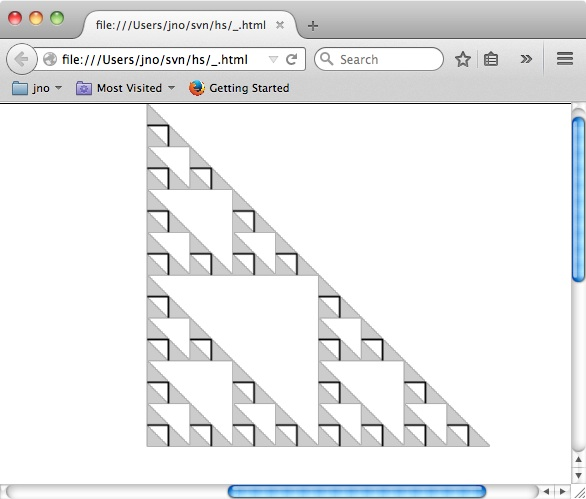
\includegraphics[width=0.6\textwidth]{media/sierp2.jpg}
\end{center}
  \caption{Um \sierp{triângulo de Sierpinski} em x3dom}\label{fig:sierp2}
\end{figure}

\subsection*{Valorização}

Se tiver tempo, investigue como é que a sua resolução desta parte do trabalho
evolui para o desenho, não de \emph{triângulos} de Sierpinski, mas sim de
\emph{pirâmides} de Sierpinski --- ver a imagem da figura \ref{fig:sierp3}.
Pode recorrer, se desejar, às funções disponibilizadas no anexo \ref{sec:X3DOM}.

\begin{figure}
\begin{center}
	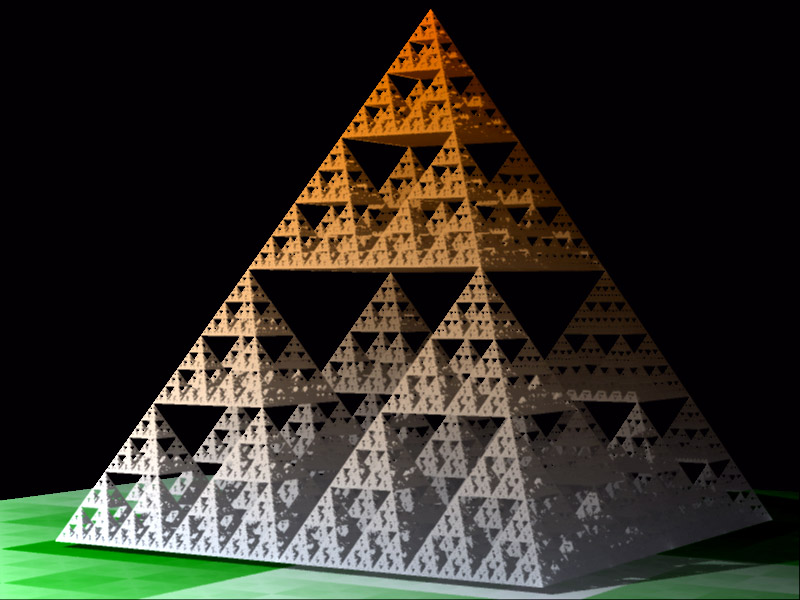
\includegraphics[width=0.6\textwidth]{media/pdSierpinski.jpg}
\end{center}
	\caption{Uma \psierp{pirâmide de Sierpinski}}\label{fig:sierp3}
\end{figure}

\section{Parte C}
\subsection{Mónades}
Os mónades são functores com propriedades adicionais que nos permitem obter
efeitos especiais em programação. Por exemplo, a biblioteca \Probability\
oferece um mónade para abordar problemas de probabilidades. Nesta biblioteca,
o conceito de distribuição estatística é captado pelo tipo
\begin{hscode}\SaveRestoreHook
\column{B}{@{}>{\hspre}l<{\hspost}@{}}%
\column{E}{@{}>{\hspre}l<{\hspost}@{}}%
\>[B]{}\mathbf{newtype}\;\Conid{Dist}\;\Varid{a}\mathrel{=}\Conid{D}\;\{\mskip1.5mu \Varid{unD}\mathbin{::}[\mskip1.5mu (\Varid{a},\Conid{ProbRep})\mskip1.5mu]\mskip1.5mu\}{}\<[E]%
\ColumnHook
\end{hscode}\resethooks
em que \ensuremath{\Conid{ProbRep}} é um real de \ensuremath{\mathrm{0}} a \ensuremath{\mathrm{1}}, equivalente a uma escala de \ensuremath{\mathrm{0}} a \ensuremath{\mathrm{100}\mathbin{\%}}.

Cada par \ensuremath{(\Varid{a},\Varid{p})} numa distribuição \ensuremath{\Varid{d}\mathbin{::}\Conid{Dist}\;\Varid{a}} indica que a probabilidade
de \ensuremath{\Varid{a}} é \ensuremath{\Varid{p}}, devendo ser garantida a propriedade de  que todas as probabilidades
de \ensuremath{\Varid{d}} somam \ensuremath{\mathrm{100}\mathbin{\%}}.
Por exemplo, a seguinte distribuição de classificações por escalões de $A$ a $E$,
\[
\begin{array}{ll}
A & \rule{2mm}{3pt}\ 2\%\\
B & \rule{12mm}{3pt}\ 12\%\\
C & \rule{29mm}{3pt}\ 29\%\\
D & \rule{35mm}{3pt}\ 35\%\\
E & \rule{22mm}{3pt}\ 22\%\\
\end{array}
\]
será representada pela distribuição
\begin{hscode}\SaveRestoreHook
\column{B}{@{}>{\hspre}l<{\hspost}@{}}%
\column{E}{@{}>{\hspre}l<{\hspost}@{}}%
\>[B]{}\Varid{d1}\mathbin{::}\Conid{Dist}\;\Conid{Char}{}\<[E]%
\\
\>[B]{}\Varid{d1}\mathrel{=}\Conid{D}\;[\mskip1.5mu (\text{\tt 'A'},\mathrm{0.02}),(\text{\tt 'B'},\mathrm{0.12}),(\text{\tt 'C'},\mathrm{0.29}),(\text{\tt 'D'},\mathrm{0.35}),(\text{\tt 'E'},\mathrm{0.22})\mskip1.5mu]{}\<[E]%
\ColumnHook
\end{hscode}\resethooks
que o \GHCi\ mostrará assim:
\begin{Verbatim}[fontsize=\small]
'D'  35.0%
'C'  29.0%
'E'  22.0%
'B'  12.0%
'A'   2.0%
\end{Verbatim}
É possível definir geradores de distribuições, por exemplo distribuições \emph{uniformes},
\begin{hscode}\SaveRestoreHook
\column{B}{@{}>{\hspre}l<{\hspost}@{}}%
\column{E}{@{}>{\hspre}l<{\hspost}@{}}%
\>[B]{}\Varid{d2}\mathrel{=}\Varid{uniform}\;(\Varid{words}\;\text{\tt \char34 Uma~frase~de~cinco~palavras\char34}){}\<[E]%
\ColumnHook
\end{hscode}\resethooks
isto é
\begin{Verbatim}[fontsize=\small]
     "Uma"  20.0%
   "cinco"  20.0%
      "de"  20.0%
   "frase"  20.0%
"palavras"  20.0%
\end{Verbatim}
distribuição \emph{normais}, eg.\
\begin{hscode}\SaveRestoreHook
\column{B}{@{}>{\hspre}l<{\hspost}@{}}%
\column{E}{@{}>{\hspre}l<{\hspost}@{}}%
\>[B]{}\Varid{d3}\mathrel{=}\Varid{normal}\;[\mskip1.5mu \mathrm{10}\mathinner{\ldotp\ldotp}\mathrm{20}\mskip1.5mu]{}\<[E]%
\ColumnHook
\end{hscode}\resethooks
etc.\footnote{Para mais detalhes ver o código fonte de \Probability, que é uma adaptação da
biblioteca \PFP\ (``Probabilistic Functional Programming''). A quem quiser souber mais
recomenda-se a leitura do artigo \cite{EK06}.}

\ensuremath{\Conid{Dist}} forma um \textbf{mónade} cuja unidade é \ensuremath{\Varid{return}\;\Varid{a}\mathrel{=}\Conid{D}\;[\mskip1.5mu (\Varid{a},\mathrm{1})\mskip1.5mu]} e cuja multiplicação é dada por
(simplificando a notação)
\begin{hscode}\SaveRestoreHook
\column{B}{@{}>{\hspre}l<{\hspost}@{}}%
\column{3}{@{}>{\hspre}l<{\hspost}@{}}%
\column{E}{@{}>{\hspre}l<{\hspost}@{}}%
\>[3]{}(\Varid{f}\kcomp \Varid{g})\;\Varid{a}\mathrel{=}[\mskip1.5mu (\Varid{y},\Varid{q}\mathbin{*}\Varid{p})\mid (\Varid{x},\Varid{p})\leftarrow \Varid{g}\;\Varid{a},(\Varid{y},\Varid{q})\leftarrow \Varid{f}\;\Varid{x}\mskip1.5mu]{}\<[E]%
\ColumnHook
\end{hscode}\resethooks
em que \ensuremath{\Varid{g}\mathbin{:}\Conid{A}\to \Conid{Dist}\;\mathit B} e \ensuremath{\Varid{f}\mathbin{:}\mathit B\to \Conid{Dist}\;\mathit C} são funções \textbf{monádicas} que representam
\emph{computações probabilísticas}.

Este mónade é adequado à resolução de problemas de \emph{probabilidades e
estatística} usando programação funcional, de forma elegante e como caso
particular de programação monádica. Vejamos um exemplo:
\begin{quote}
\emph{Problema: qual é a soma de faces mais provável quando lançamos dois dados num tabuleiro?}
\end{quote}
Assumindo que os dados não estão viciados, cada um oferece uma distribuição uniforme
das suas faces (\ensuremath{\mathrm{1}} a \ensuremath{\mathrm{6}}). Basta correr a expressão monádica
\begin{quote}
\ensuremath{\mathbf{do}\;\{\mskip1.5mu \Varid{x}\leftarrow \Varid{uniform}\;[\mskip1.5mu \mathrm{1}\mathinner{\ldotp\ldotp}\mathrm{6}\mskip1.5mu];\Varid{y}\leftarrow \Varid{uniform}\;[\mskip1.5mu \mathrm{1}\mathinner{\ldotp\ldotp}\mathrm{6}\mskip1.5mu];\Varid{return}\;(\Varid{x}\mathbin{+}\Varid{y})\mskip1.5mu\}}
\end{quote}
e obter-se-á:
\begin{Verbatim}[fontsize=\small]
*Main> do { x <- uniform [1..6] ;  y <- uniform [1..6] ; return(x+y) }
 7  16.7%
 6  13.9%
 8  13.9%
 5  11.1%
 9  11.1%
 4   8.3%
10   8.3%
 3   5.6%
11   5.6%
 2   2.8%
12   2.8%
\end{Verbatim}
A soma mais provável é \ensuremath{\mathrm{7}}, com \ensuremath{\mathrm{16.7}\mathbin{\%}}.

\subsection{Trabalho a realizar}\label{sec:monads}
É possível pensarmos em catamorfismos, anamorfismos etc probabilísticos,
quer dizer, programas recursivos que dão distribuições como resultados. Por
exemplo, neste enunciado é dado o combinador
\begin{hscode}\SaveRestoreHook
\column{B}{@{}>{\hspre}l<{\hspost}@{}}%
\column{E}{@{}>{\hspre}l<{\hspost}@{}}%
\>[B]{}\Varid{pcataList}\mathbin{::}(\Conid{Either}\;()\;(\Varid{a},\Varid{b})\to \Conid{Dist}\;\Varid{b})\to [\mskip1.5mu \Varid{a}\mskip1.5mu]\to \Conid{Dist}\;\Varid{b}{}\<[E]%
\ColumnHook
\end{hscode}\resethooks
que é muito parecido com
\begin{hscode}\SaveRestoreHook
\column{B}{@{}>{\hspre}l<{\hspost}@{}}%
\column{E}{@{}>{\hspre}l<{\hspost}@{}}%
\>[B]{}\Varid{cataList}\mathbin{::}(\Conid{Either}\;()\;(\Varid{a},\Varid{b})\to \Varid{b})\to [\mskip1.5mu \Varid{a}\mskip1.5mu]\to \Varid{b}{}\<[E]%
\ColumnHook
\end{hscode}\resethooks
da biblioteca \List. A única diferença é que o gene de \ensuremath{\Varid{pcataList}} é uma função probabilística.

Exemplo de utilização: recorde-se que \ensuremath{\Varid{cataList}\;\alt{\Varid{zero}}{\Varid{add}}} soma todos
os elementos da lista argumento, por exemplo:
\begin{quote}
\ensuremath{\Varid{cataList}\;\alt{\Varid{zero}}{\Varid{add}}\;[\mskip1.5mu \mathrm{20},\mathrm{10},\mathrm{5}\mskip1.5mu]\mathrel{=}\mathrm{35}}.
\end{quote}
Considere agora a função \ensuremath{\Varid{padd}} (adição probabilística) que,
com probabilidade \ensuremath{\mathrm{90}\mathbin{\%}} soma dois números e com probabilidade \ensuremath{\mathrm{10}\mathbin{\%}} os subtrai:
\begin{hscode}\SaveRestoreHook
\column{B}{@{}>{\hspre}l<{\hspost}@{}}%
\column{E}{@{}>{\hspre}l<{\hspost}@{}}%
\>[B]{}\Varid{padd}\;(\Varid{a},\Varid{b})\mathrel{=}\Conid{D}\;[\mskip1.5mu (\Varid{a}\mathbin{+}\Varid{b},\mathrm{0.9}),(\Varid{a}\mathbin{-}\Varid{b},\mathrm{0.1})\mskip1.5mu]{}\<[E]%
\ColumnHook
\end{hscode}\resethooks
Se se correr
\begin{hscode}\SaveRestoreHook
\column{B}{@{}>{\hspre}l<{\hspost}@{}}%
\column{E}{@{}>{\hspre}l<{\hspost}@{}}%
\>[B]{}\Varid{d4}\mathrel{=}\Varid{pcataList}\;\alt{\Varid{pzero}}{\Varid{padd}}\;[\mskip1.5mu \mathrm{20},\mathrm{10},\mathrm{5}\mskip1.5mu]\;\mathbf{where}\;\Varid{pzero}\mathrel{=}\Varid{return}\comp \Varid{zero}{}\<[E]%
\ColumnHook
\end{hscode}\resethooks
obter-se-á:
\begin{Verbatim}[fontsize=\small]
35  81.0%
25   9.0%
 5   9.0%
15   1.0%
\end{Verbatim}

Com base nestes exemplos, resolva o seguinte
\begin{quote}\em
\textbf{Problema}: Uma unidade militar pretende enviar uma mensagem urgente
a outra, mas tem o aparelho de telegrafia meio avariado. Por experiência,
o telegrafista sabe que a probabilidade de uma palavra se perder (não ser
transmitida) é \ensuremath{\mathrm{5}\mathbin{\%}}; no final de cada mensagem, o aparelho envia o código
\ensuremath{\text{\tt \char34 stop\char34}}, mas (por estar meio avariado), falha \ensuremath{\mathrm{10}\mathbin{\%}} das vezes.

Qual a probabilidade de a palavra \ensuremath{\text{\tt \char34 atacar\char34}} da mensagem \ensuremath{\Varid{words}\;\text{\tt \char34 Vamos~atacar~hoje\char34}} se perder, isto é, o resultado da transmissão ser \ensuremath{[\mskip1.5mu \text{\tt \char34 Vamos\char34},\text{\tt \char34 hoje\char34},\text{\tt \char34 stop\char34}\mskip1.5mu]}?
e a de seguirem todas as palavras, mas faltar o \ensuremath{\text{\tt \char34 stop\char34}} no fim? E a da transmissão
ser perfeita?
\end{quote}

Responda a todas estas perguntas encontrando \ensuremath{\Varid{g}} tal que
\begin{hscode}\SaveRestoreHook
\column{B}{@{}>{\hspre}l<{\hspost}@{}}%
\column{E}{@{}>{\hspre}l<{\hspost}@{}}%
\>[B]{}\Varid{transmitir}\mathrel{=}\Varid{pcataList}\;\Varid{gene}{}\<[E]%
\ColumnHook
\end{hscode}\resethooks
descreve o comportamento do aparelho.
%
\begin{teste}
Faça o seguinte teste unitário da sua versão para \ensuremath{\Varid{gene}}:
\begin{hscode}\SaveRestoreHook
\column{B}{@{}>{\hspre}l<{\hspost}@{}}%
\column{E}{@{}>{\hspre}l<{\hspost}@{}}%
\>[B]{}\Varid{test07}\mathrel{=}\Varid{gene}\;(i_2\;(\text{\tt \char34 a\char34},[\mskip1.5mu \text{\tt \char34 b\char34}\mskip1.5mu]))\equiv \Conid{D}\;[\mskip1.5mu ([\mskip1.5mu \text{\tt \char34 a\char34},\text{\tt \char34 b\char34}\mskip1.5mu],\mathrm{0.95}),([\mskip1.5mu \text{\tt \char34 b\char34}\mskip1.5mu],\mathrm{0.05})\mskip1.5mu]{}\<[E]%
\ColumnHook
\end{hscode}\resethooks
\end{teste}
Responda então às perguntas do problema acima correndo a expressão:
\begin{quote}
\ensuremath{\Varid{transmitir}\;(\Varid{words}\;\text{\tt \char34 Vamos~atacar~hoje\char34})}
\end{quote}

\subsection{Programação funcional paralela}
Uma outra aplicação do conceito de mónade é a programação funcional paralela.
A biblioteca \ControlParallelStrategies, já carregada no início deste texto,
implementa esse tipo de programação, que hoje está na ordem do dia. O mónade
respectivo chama-se \ensuremath{\Conid{Eval}} e disponibiliza duas funções,
\begin{hscode}\SaveRestoreHook
\column{B}{@{}>{\hspre}l<{\hspost}@{}}%
\column{E}{@{}>{\hspre}l<{\hspost}@{}}%
\>[B]{}\Varid{rpar}\mathbin{::}\Varid{a}\to \Conid{Eval}\;\Varid{a}{}\<[E]%
\\
\>[B]{}\Varid{rseq}\mathbin{::}\Varid{a}\to \Conid{Eval}\;\Varid{a}{}\<[E]%
\ColumnHook
\end{hscode}\resethooks
conforme se deseja que uma dada computação seja efectuada em paralelo ou
sequencialmente.\footnote{Esta explicação é bastante simplista, mas serve
de momento. Para uma abordagem completa e elucidativa ver a referência \cite{Ma13}.}
Por exemplo,
\begin{hscode}\SaveRestoreHook
\column{B}{@{}>{\hspre}l<{\hspost}@{}}%
\column{5}{@{}>{\hspre}l<{\hspost}@{}}%
\column{E}{@{}>{\hspre}l<{\hspost}@{}}%
\>[B]{}\Varid{parmap}\mathbin{::}(\Varid{a}\to \Varid{b})\to [\mskip1.5mu \Varid{a}\mskip1.5mu]\to \Conid{Eval}\;[\mskip1.5mu \Varid{b}\mskip1.5mu]{}\<[E]%
\\
\>[B]{}\Varid{parmap}\;\Varid{f}\;[\mskip1.5mu \mskip1.5mu]\mathrel{=}\Varid{return}\;[\mskip1.5mu \mskip1.5mu]{}\<[E]%
\\
\>[B]{}\Varid{parmap}\;\Varid{f}\;(\Varid{a}\mathbin{:}\Varid{lt})\mathrel{=}\mathbf{do}{}\<[E]%
\\
\>[B]{}\hsindent{5}{}\<[5]%
\>[5]{}\Varid{a'}\leftarrow \Varid{rpar}\;(\Varid{f}\;\Varid{a}){}\<[E]%
\\
\>[B]{}\hsindent{5}{}\<[5]%
\>[5]{}\Varid{lt'}\leftarrow \Varid{parmap}\;\Varid{f}\;\Varid{lt}{}\<[E]%
\\
\>[B]{}\hsindent{5}{}\<[5]%
\>[5]{}\Varid{return}\;(\Varid{a'}\mathbin{:}\Varid{lt'}){}\<[E]%
\ColumnHook
\end{hscode}\resethooks
é um \ensuremath{\Varid{map}} monádico que usa \ensuremath{\Varid{rpar}} para aplicar \ensuremath{\Varid{f}} a todos os elementos
de uma lista \emph{em paralelo}.

Se corrermos o \ensuremath{\Varid{map}} habitual em
\begin{quote}
\ensuremath{\Varid{map}\;\Varid{fib}\;[\mskip1.5mu \mathrm{20}\mathinner{\ldotp\ldotp}\mathrm{30}\mskip1.5mu]\mathrel{=}[\mskip1.5mu \mathrm{10946},\mathrm{17711},\mathrm{28657},\mathrm{46368},\mathrm{75025},\mathrm{121393},\mathrm{196418},\mathrm{317811},\mathrm{514229},\mathrm{832040},\mathrm{1346269}\mskip1.5mu]}
\end{quote}
(cálculo dos números de Fibonacci do vigésimo ao trigésimo), o tempo que
o cálculo vai demorar numa máquina com 2 cores\footnote{Intel Core 2 Duo
a 2.53 GHz.} será da ordem de \ensuremath{\mathrm{1.1}}s. Já no caso de usar \ensuremath{\Varid{parmap}}
em vez de \ensuremath{\Varid{map}}, fará o mesmo cálculo em cerca de \ensuremath{\mathrm{60}\mathbin{\%}} desse tempo.

Para verificar esta diferença siga as instruções seguintes:\footnote{Ver detalhes em \cite{Ma13}.}
\begin{enumerate}
\item	Compile o presente enunciado correndo:
\begin{tabbing}\tt
~ghc~\char45{}O2~cp1415t~\char45{}rtsopts~\char45{}threaded
\end{tabbing}
\item	De seguida execute numa ``shell'' o seguinte comando,
\begin{tabbing}\tt
~\char46{}\char47{}cp1415t~exemplo~seq~\char43{}RTS~\char45{}s~\char45{}N2
\end{tabbing}
onde o \ensuremath{\mathrm{2}} em \ensuremath{\Conid{N2}} indica \ensuremath{\mathrm{2}} \emph{cores} (se a máquina em questão tiver
mais \emph{cores}, este número deverá ser actualizado). Como pode ver inspecionando
o código da função \ensuremath{\Varid{main}} na secção \ref{sec:main}, o que vai ser executado é
\begin{hscode}\SaveRestoreHook
\column{B}{@{}>{\hspre}l<{\hspost}@{}}%
\column{E}{@{}>{\hspre}l<{\hspost}@{}}%
\>[B]{}\Varid{putStrLn}\comp \Varid{show}\comp (\Varid{map}\;\Varid{fib})\mathbin{\$}[\mskip1.5mu \mathrm{20}\mathinner{\ldotp\ldotp}\mathrm{30}\mskip1.5mu]{}\<[E]%
\ColumnHook
\end{hscode}\resethooks
Das estatísticas que lhe aparecem no écran retenha esta:
\begin{tabbing}\tt
~Total~~~time~~~~1\char46{}41s~~\char40{}~~1\char46{}11s~elapsed\char41{}
\end{tabbing}
Em particular, o campo \ensuremath{\Varid{elapsed}} apresenta o tempo decorrido desde o início
da execução do programa até ao respectivo fim.
\item	De seguida execute
\begin{tabbing}\tt
~\char46{}\char47{}cp1415t~exemplo~par~\char43{}RTS~\char45{}s~\char45{}N2
\end{tabbing}
que irá chamar, desta vez
\begin{hscode}\SaveRestoreHook
\column{B}{@{}>{\hspre}l<{\hspost}@{}}%
\column{E}{@{}>{\hspre}l<{\hspost}@{}}%
\>[B]{}\Varid{putStrLn}\comp \Varid{show}\comp \Varid{runEval}\comp (\Varid{parmap}\;\Varid{fib})\mathbin{\$}[\mskip1.5mu \mathrm{20}\mathinner{\ldotp\ldotp}\mathrm{30}\mskip1.5mu]{}\<[E]%
\ColumnHook
\end{hscode}\resethooks
A estatística correspondente à de cima será, desta vez, da ordem seguinte:
\begin{tabbing}\tt
~Total~~~time~~~~1\char46{}13s~~\char40{}~~0\char46{}69s~elapsed\char41{}
\end{tabbing}
Em suma, a versão paralela é cerca de 1.61x mais rápida \ensuremath{(\frac{\mathrm{1.11}}{\mathrm{0.69}})}
que a sequencial.
\end{enumerate}

\subsection{Trabalho a realizar}\label{sec:parBTreeMap}
Com base na definição de \ensuremath{\Varid{parmap}} acima,
defina a função
\begin{hscode}\SaveRestoreHook
\column{B}{@{}>{\hspre}l<{\hspost}@{}}%
\column{E}{@{}>{\hspre}l<{\hspost}@{}}%
\>[B]{}\Varid{parBTreeMap}\mathbin{::}(\Varid{a}\to \Varid{b})\to (\Conid{BTree}\;\Varid{a})\to \Conid{Eval}\;(\Conid{BTree}\;\Varid{b}){}\<[E]%
\ColumnHook
\end{hscode}\resethooks
que implemente o ``map paralelo'' sobre \BTree's.

De seguida, corra testes semelhantes aos apresentados acima para apurar o ganho
em \emph{performance} da aplicação da função \ensuremath{\Varid{fib}} a todos os números
da árvore \ensuremath{\Varid{t1}} da secção \ref{sec:BTree}, em duas versões:
\begin{enumerate}
\item \ensuremath{\Varid{fmap}\;\Varid{fib}} (sem paralelismo, usando a função definida em \BTree), ou
\item usando \ensuremath{\Varid{parBTreeMap}\;\Varid{fib}}.
\end{enumerate}
Em máquinas mais rápidas e/ou com mais ``cores'' deve usar números maiores para obter
uma melhor distinção entre as duas versões.

%----------------- Bibliografia (exige bibtex) --------------------------------%

\bibliographystyle{plain}
\bibliography{cp1415t}

%----------------- Programa, bibliotecas e código auxiliar --------------------%

\newpage

\part*{Anexos}

\appendix

\section{Programa principal}\label{sec:main}
\begin{hscode}\SaveRestoreHook
\column{B}{@{}>{\hspre}l<{\hspost}@{}}%
\column{6}{@{}>{\hspre}l<{\hspost}@{}}%
\column{9}{@{}>{\hspre}l<{\hspost}@{}}%
\column{E}{@{}>{\hspre}l<{\hspost}@{}}%
\>[B]{}\Varid{main}\mathbin{::}\Conid{IO}\;(){}\<[E]%
\\
\>[B]{}\Varid{main}\mathrel{=}\Varid{getArgs}\bind \mcond{(\neg \comp \Varid{null})}{\Varid{exemp\char95 or\char95 exer}}{\Varid{errInvArgs}}{}\<[E]%
\\
\>[B]{}\hsindent{6}{}\<[6]%
\>[6]{}\mathbf{where}{}\<[E]%
\\
\>[6]{}\hsindent{3}{}\<[9]%
\>[9]{}\Varid{exemp\char95 or\char95 exer}\mathrel{=}\mcond{(((\equiv )\;\text{\tt \char34 exemplo\char34})\comp \Varid{head})}{\Varid{exemp}}{\Varid{exer}}{}\<[E]%
\\
\>[6]{}\hsindent{3}{}\<[9]%
\>[9]{}\Varid{exemp}\mathrel{=}\mcond{(((\equiv )\;\mathrm{2})\comp \Varid{length})}{\Varid{execExemp}}{\Varid{errInvArgs}}{}\<[E]%
\\
\>[6]{}\hsindent{3}{}\<[9]%
\>[9]{}\Varid{execExemp}\mathrel{=}\mcond{\Varid{isPar}}{\Varid{execExempPar}}{\Varid{execExempSeq}}{}\<[E]%
\\
\>[6]{}\hsindent{3}{}\<[9]%
\>[9]{}\Varid{exer}\mathrel{=}\mcond{(((\equiv )\;\mathrm{3})\comp \Varid{length})}{\Varid{execExer}}{\Varid{errInvArgs}}{}\<[E]%
\\
\>[6]{}\hsindent{3}{}\<[9]%
\>[9]{}\Varid{execExer}\mathrel{=}\mcond{\Varid{isPar}}{\Varid{execExerPar}}{\Varid{execExerSeq}}{}\<[E]%
\\
\>[6]{}\hsindent{3}{}\<[9]%
\>[9]{}\Varid{execExempSeq}\mathrel{=}\underline{(\Varid{putStrLn}\comp \Varid{show}\comp (\Varid{map}\;\Varid{fib})\mathbin{\$}[\mskip1.5mu \mathrm{20}\mathinner{\ldotp\ldotp}\mathrm{30}\mskip1.5mu])}{}\<[E]%
\\
\>[6]{}\hsindent{3}{}\<[9]%
\>[9]{}\Varid{execExempPar}\mathrel{=}\underline{(\Varid{putStrLn}\comp \Varid{show}\comp \Varid{runEval}\comp (\Varid{parmap}\;\Varid{fib})\mathbin{\$}[\mskip1.5mu \mathrm{20}\mathinner{\ldotp\ldotp}\mathrm{30}\mskip1.5mu])}{}\<[E]%
\ColumnHook
\end{hscode}\resethooks

\section{Bibliotecas e código auxiliar}
\begin{hscode}\SaveRestoreHook
\column{B}{@{}>{\hspre}l<{\hspost}@{}}%
\column{5}{@{}>{\hspre}l<{\hspost}@{}}%
\column{12}{@{}>{\hspre}l<{\hspost}@{}}%
\column{14}{@{}>{\hspre}l<{\hspost}@{}}%
\column{E}{@{}>{\hspre}l<{\hspost}@{}}%
\>[B]{}\Varid{errInvArgs}\mathbin{::}\Varid{a}\to \Conid{IO}\;(){}\<[E]%
\\
\>[B]{}\Varid{errInvArgs}\mathrel{=}\underline{\cdot }\mathbin{\$}\Varid{putStrLn}\;\Varid{msgInvArgs}{}\<[E]%
\\
\>[B]{}\hsindent{12}{}\<[12]%
\>[12]{}\mathbf{where}{}\<[E]%
\\
\>[B]{}\hsindent{12}{}\<[12]%
\>[12]{}\Varid{msgInvArgs}\mathrel{=}\text{\tt \char34 Invalid~arguments\char34}{}\<[E]%
\\[\blanklineskip]%
\>[B]{}\Varid{execExerPar}\mathbin{::}[\mskip1.5mu \Conid{String}\mskip1.5mu]\to \Conid{IO}\;(){}\<[E]%
\\
\>[B]{}\Varid{execExerPar}{}\<[14]%
\>[14]{}\mathrel{=}\bot {}\<[E]%
\\[\blanklineskip]%
\>[B]{}\Varid{execExerSeq}\mathbin{::}[\mskip1.5mu \Conid{String}\mskip1.5mu]\to \Conid{IO}\;(){}\<[E]%
\\
\>[B]{}\Varid{execExerSeq}\mathrel{=}\bot {}\<[E]%
\\[\blanklineskip]%
\>[B]{}\Varid{isPar}\mathbin{::}[\mskip1.5mu \Conid{String}\mskip1.5mu]\to \Conid{Bool}{}\<[E]%
\\
\>[B]{}\Varid{isPar}\mathrel{=}\mcond{(((\equiv )\;\text{\tt \char34 par\char34})\comp \Varid{head}\comp \Varid{tail})}{\underline{\Conid{True}}}{\underline{\Conid{False}}}{}\<[E]%
\\[\blanklineskip]%
\>[B]{}\Varid{pcataList}\;\Varid{g}\mathrel{=}\Varid{mfoldr}\;(\Varid{curry}\;(\Varid{g}\comp i_2))\;((\Varid{g}\comp i_1)\;())\;\mathbf{where}{}\<[E]%
\\
\>[B]{}\hsindent{5}{}\<[5]%
\>[5]{}\Varid{mfoldr}\;\Varid{f}\;\Varid{d}\;[\mskip1.5mu \mskip1.5mu]\mathrel{=}\Varid{d}{}\<[E]%
\\
\>[B]{}\hsindent{5}{}\<[5]%
\>[5]{}\Varid{mfoldr}\;\Varid{f}\;\Varid{d}\;(\Varid{a}\mathbin{:}\Varid{x})\mathrel{=}\mathbf{do}\;\{\mskip1.5mu \Varid{y}\leftarrow \Varid{mfoldr}\;\Varid{f}\;\Varid{d}\;\Varid{x};\Varid{f}\;\Varid{a}\;\Varid{y}\mskip1.5mu\}{}\<[E]%
\ColumnHook
\end{hscode}\resethooks

\subsection{``Easy X3DOM access''}\label{sec:X3DOM}
Defina-se a seguinte composição de funções
\begin{hscode}\SaveRestoreHook
\column{B}{@{}>{\hspre}l<{\hspost}@{}}%
\column{E}{@{}>{\hspre}l<{\hspost}@{}}%
\>[B]{}\Varid{x3dom}\mathrel{=}\Varid{html}\comp \Varid{preamble}\comp \Varid{body}\comp \Varid{x3d}\comp \Varid{scene}\comp \Varid{items}{}\<[E]%
\ColumnHook
\end{hscode}\resethooks
para gerar um texto HTML que represente um objecto gráfico em \XFreedom.
Esta função usa as seguintes funções auxiliares:
\begin{hscode}\SaveRestoreHook
\column{B}{@{}>{\hspre}l<{\hspost}@{}}%
\column{5}{@{}>{\hspre}l<{\hspost}@{}}%
\column{E}{@{}>{\hspre}l<{\hspost}@{}}%
\>[B]{}\Varid{html}\mathrel{=}\Varid{tag}\;\text{\tt \char34 html\char34}\;[\mskip1.5mu \mskip1.5mu]{}\<[E]%
\\[\blanklineskip]%
\>[B]{}\Varid{preamble}\mathrel{=}\Varid{headx}\mathbin{`\Varid{with}`}[\mskip1.5mu \Varid{title}\;\text{\tt \char34 CP/X3DOM~generation\char34},\Varid{links},\Varid{script}\mskip1.5mu]{}\<[E]%
\\[\blanklineskip]%
\>[B]{}\Varid{body}\mathrel{=}\Varid{tag}\;\text{\tt \char34 body\char34}\;[\mskip1.5mu \mskip1.5mu]{}\<[E]%
\\[\blanklineskip]%
\>[B]{}\Varid{x3d}\mathrel{=}\Varid{tag}\;\text{\tt \char34 x3d\char34}\;[\mskip1.5mu (\text{\tt \char34 width\char34},\text{\tt \char34 \char92 \char34 500px\char92 \char34 \char34}),(\text{\tt \char34 height\char34},\text{\tt \char34 \char92 \char34 400px\char92 \char34 \char34})\mskip1.5mu]{}\<[E]%
\\[\blanklineskip]%
\>[B]{}\Varid{scene}\mathrel{=}\Varid{tag}\;\text{\tt \char34 scene\char34}\;[\mskip1.5mu \mskip1.5mu]{}\<[E]%
\\[\blanklineskip]%
\>[B]{}\Varid{items}\mathrel{=}\Varid{concat}{}\<[E]%
\\[\blanklineskip]%
\>[B]{}\Varid{links}\mathrel{=}\Varid{ctag}\;\text{\tt \char34 link\char34}\;[\mskip1.5mu {}\<[E]%
\\
\>[B]{}\hsindent{5}{}\<[5]%
\>[5]{}(\text{\tt \char34 rel\char34},\Varid{quote}\;\text{\tt \char34 stylesheet\char34}),(\text{\tt \char34 type\char34},\Varid{quote}\;\text{\tt \char34 text/css\char34}),{}\<[E]%
\\
\>[B]{}\hsindent{5}{}\<[5]%
\>[5]{}(\text{\tt \char34 href\char34},\Varid{quote}\;\text{\tt \char34 http://www.x3dom.org/x3dom/release/x3dom.css\char34})\mskip1.5mu]{}\<[E]%
\\[\blanklineskip]%
\>[B]{}\Varid{script}\mathrel{=}\Varid{ctag}\;\text{\tt \char34 script\char34}\;[\mskip1.5mu {}\<[E]%
\\
\>[B]{}\hsindent{5}{}\<[5]%
\>[5]{}(\text{\tt \char34 type\char34},\Varid{quote}\;\text{\tt \char34 text/javascript\char34}),{}\<[E]%
\\
\>[B]{}\hsindent{5}{}\<[5]%
\>[5]{}(\text{\tt \char34 src\char34},\Varid{quote}\;\text{\tt \char34 http://www.x3dom.org/x3dom/release/x3dom.js\char34})\mskip1.5mu]{}\<[E]%
\\[\blanklineskip]%
\>[B]{}\Varid{ctag}\;\Varid{t}\;\Varid{l}\mathrel{=}\Varid{tag}\;\Varid{t}\;\Varid{l}\;\text{\tt \char34 \char34}{}\<[E]%
\ColumnHook
\end{hscode}\resethooks
onde
\begin{hscode}\SaveRestoreHook
\column{B}{@{}>{\hspre}l<{\hspost}@{}}%
\column{6}{@{}>{\hspre}l<{\hspost}@{}}%
\column{E}{@{}>{\hspre}l<{\hspost}@{}}%
\>[B]{}\Varid{tag}\;\Varid{t}\;\Varid{l}\;\Varid{x}\mathrel{=}\text{\tt \char34 <\char34}\plus \Varid{t}\plus \text{\tt \char34 ~\char34}\plus \Varid{ps}\plus \text{\tt \char34 >\char34}\plus \Varid{x}\plus \text{\tt \char34 </\char34}\plus \Varid{t}\plus \text{\tt \char34 >\char34}{}\<[E]%
\\
\>[B]{}\hsindent{6}{}\<[6]%
\>[6]{}\mathbf{where}\;\Varid{ps}\mathrel{=}\Varid{unwords}\;[\mskip1.5mu \Varid{concat}\;[\mskip1.5mu \Varid{t},\text{\tt \char34 =\char34},\Varid{v}\mskip1.5mu]\mid (\Varid{t},\Varid{v})\leftarrow \Varid{l}\mskip1.5mu]{}\<[E]%
\\[\blanklineskip]%
\>[B]{}\Varid{headx}\mathrel{=}\Varid{tag}\;\text{\tt \char34 head\char34}\;[\mskip1.5mu \mskip1.5mu]{}\<[E]%
\ColumnHook
\end{hscode}\resethooks
De seguida dão-se mais algumas funções auxiliares facilitadoras:
\begin{hscode}\SaveRestoreHook
\column{B}{@{}>{\hspre}l<{\hspost}@{}}%
\column{10}{@{}>{\hspre}l<{\hspost}@{}}%
\column{12}{@{}>{\hspre}l<{\hspost}@{}}%
\column{E}{@{}>{\hspre}l<{\hspost}@{}}%
\>[B]{}\Varid{transform}\;(\Varid{x},\Varid{y},\Varid{z})\mathrel{=}\Varid{tag}\;\text{\tt \char34 transform\char34}\;[\mskip1.5mu (\text{\tt \char34 translation\char34},\Varid{quote}\;(\Varid{show3D}\;(\Varid{x},\Varid{y},\Varid{x})))\mskip1.5mu]{}\<[E]%
\\[\blanklineskip]%
\>[B]{}\Varid{groupx}\;(\Varid{x},\Varid{y},\Varid{z})\mathrel{=}(\Varid{tag}\;\text{\tt \char34 group\char34}\;[\mskip1.5mu (\text{\tt \char34 bboxSize\char34},\Varid{quote}\;(\Varid{show3D}\;(\Varid{x},\Varid{y},\Varid{z})))\mskip1.5mu])\comp \Varid{items}{}\<[E]%
\\[\blanklineskip]%
\>[B]{}\Varid{shapex}\mathrel{=}\Varid{tag}\;\text{\tt \char34 shape\char34}\;[\mskip1.5mu \mskip1.5mu]{}\<[E]%
\\[\blanklineskip]%
\>[B]{}\Varid{title}\mathrel{=}\Varid{tag}\;\text{\tt \char34 title\char34}\;[\mskip1.5mu \mskip1.5mu]{}\<[E]%
\\[\blanklineskip]%
\>[B]{}\Varid{appearance}\mathrel{=}\Varid{tag}\;\text{\tt \char34 appearance\char34}\;[\mskip1.5mu \mskip1.5mu]{}\<[E]%
\\[\blanklineskip]%
\>[B]{}\Varid{show3D}\;(\Varid{x},\Varid{y},\Varid{z})\mathrel{=}\Varid{show}\;\Varid{x}\plus \text{\tt \char34 ~\char34}\plus \Varid{show}\;\Varid{y}\plus \text{\tt \char34 ~\char34}\plus \Varid{show}\;\Varid{z}{}\<[E]%
\\[\blanklineskip]%
\>[B]{}\Varid{t}\mathbin{`\Varid{with}`}\Varid{l}\mathrel{=}((\Varid{t}\mathbin{\$}\Varid{items}\;\Varid{l})\plus ){}\<[E]%
\\[\blanklineskip]%
\>[B]{}\Varid{quote}\;\Varid{s}\mathrel{=}\text{\tt \char34 \char92 \char34 \char34}\plus \Varid{s}\plus \text{\tt \char34 \char92 \char34 \char34}{}\<[E]%
\\[\blanklineskip]%
\>[B]{}\Varid{prime}\;\Varid{s}\mathrel{=}\text{\tt \char34 '\char34}\plus \Varid{s}\plus \text{\tt \char34 '\char34}{}\<[E]%
\\[\blanklineskip]%
\>[B]{}\Varid{box}\;\Varid{p}\;\Varid{col}\mathrel{=}(\Varid{transform}\;\Varid{p}\comp \Varid{shapex}\comp \Varid{items})\;[\mskip1.5mu \Varid{color}\;\Varid{col},\Varid{ctag}\;\text{\tt \char34 box\char34}\;[\mskip1.5mu (\text{\tt \char34 size\char34},\Varid{prime}\;\text{\tt \char34 2,2,2\char34})\mskip1.5mu]\mskip1.5mu]{}\<[E]%
\\[\blanklineskip]%
\>[B]{}\Varid{cone}\;\Varid{p}\;\Varid{col}\;\Varid{b}\;\Varid{h}\mathrel{=}(\Varid{transform}\;\Varid{p}\comp \Varid{shapex}\comp \Varid{items}){}\<[E]%
\\
\>[B]{}\hsindent{10}{}\<[10]%
\>[10]{}[\mskip1.5mu \Varid{color}\;\Varid{col},{}\<[E]%
\\
\>[10]{}\hsindent{2}{}\<[12]%
\>[12]{}\Varid{ctag}\;\text{\tt \char34 cone\char34}\;[\mskip1.5mu (\text{\tt \char34 bottomRadius\char34},\Varid{prime}\;(\Varid{show}\;\Varid{b})),(\text{\tt \char34 height\char34},\Varid{prime}\;(\Varid{show}\;\Varid{h}))\mskip1.5mu]\mskip1.5mu]{}\<[E]%
\\[\blanklineskip]%
\>[B]{}\Varid{color}\;\Varid{c}\mathrel{=}\Varid{appearance}\;(\Varid{ctag}\;\text{\tt \char34 material\char34}\;[\mskip1.5mu (\text{\tt \char34 diffuseColor\char34},\Varid{prime}\;\Varid{c})\mskip1.5mu]){}\<[E]%
\ColumnHook
\end{hscode}\resethooks

%----------------- Soluções propostas -----------------------------------------%
\section{Soluções propostas}\label{sec:resolucao}

\subsection*{Secção \ref{sec:LTree}}
A função [depth] recebe uma LTree e returna a altura da LTree. Usando um catamorfismo de um [either one (succ . uncurry max)], em que [one] é a altura da árvore que contém só uma folha e [succ] . [uncurry max] caso a árvore contenha mais que uma folha e, nessa situação, a altura é calculado através da maior arvore, esquerda ou direita.

A função [balance] usa a função [tips], que coloca todos os elementos de uma LTree numa lista com todos os elementos da mesma. Essa lista é organizada pelo anamorfismo da função [lsplit], que organiza a mesma, para depois devolver uma nova árvore, desta vez, balanceada, com os elementos da lista já organizados.
\begin{hscode}\SaveRestoreHook
\column{B}{@{}>{\hspre}l<{\hspost}@{}}%
\column{E}{@{}>{\hspre}l<{\hspost}@{}}%
\>[B]{}\Varid{depth}\mathbin{::}\Conid{LTree}\;\Varid{a}\to \Conid{Integer}{}\<[E]%
\\
\>[B]{}\Varid{depth}\mathrel{=}\Varid{cataLTree}\;\alt{\Varid{one}}{\Varid{succ}\comp \uncurry{(\Varid{max})}}{}\<[E]%
\\[\blanklineskip]%
\>[B]{}\Varid{balance}\mathbin{::}\Conid{LTree}\;\Varid{a}\to \Conid{LTree}\;\Varid{a}{}\<[E]%
\\
\>[B]{}\Varid{balance}\mathrel{=}\Varid{anaLTree}\;\Varid{lsplit}\comp \Varid{tips}{}\<[E]%
\ColumnHook
\end{hscode}\resethooks

\subsection*{Secção \ref{sec:BTree}}
A função [qsplit] corresponde a um gene e funciona como função auxiliar da [abpe].
Esta função recebe como parametro um par de dois numeros inteiros que vai ser usados para gerar uma BTree, colocando o valor medio na cabeça e criando a subarvore a esquerda com valores inferiores a cabeça e a subarvore a direita com os valores maiores.

\begin{hscode}\SaveRestoreHook
\column{B}{@{}>{\hspre}l<{\hspost}@{}}%
\column{9}{@{}>{\hspre}l<{\hspost}@{}}%
\column{E}{@{}>{\hspre}l<{\hspost}@{}}%
\>[B]{}\Varid{qsplit}\mathbin{::}\Conid{Integral}\;\Varid{a}\Rightarrow (\Varid{a},\Varid{a})\to \Conid{Either}\;()\;(\Varid{a},((\Varid{a},\Varid{a}),(\Varid{a},\Varid{a}))){}\<[E]%
\\
\>[B]{}\Varid{qsplit}\;(\Varid{x},\Varid{y})\mathrel{=}\mathbf{if}\;(\Varid{x}\mathbin{>}\Varid{y})\mathrel{\vee}(\Varid{x}\equiv \mathrm{0}\mathrel{\wedge}\Varid{y}\equiv \mathrm{0})\;\mathbf{then}\;i_1\;()\;\mathbf{else}\;i_2\;(\Varid{media},((\Varid{x},\Varid{media}\mathbin{-}\mathrm{1}),(\Varid{media}\mathbin{+}\mathrm{1},\Varid{y}))){}\<[E]%
\\
\>[B]{}\hsindent{9}{}\<[9]%
\>[9]{}\mathbf{where}\;\Varid{media}\mathrel{=}\Varid{x}\mathbin{+}\Varid{y}\div \mathrm{2}{}\<[E]%
\ColumnHook
\end{hscode}\resethooks

\subsection*{Secção \ref{sec:SList}}
Nesta secção estão presentes várias funções para a biblioteca SList, tal como estão definidas para as restantes bibliotecas. Contém também uma função [mgen], que é o gene de [merge]. 
Recebe um par de listas e parte-a, separando a cabeça da primeira lista do par com a sua cauda e com a segunda lista recebida como parâmetro. 

\begin{hscode}\SaveRestoreHook
\column{B}{@{}>{\hspre}l<{\hspost}@{}}%
\column{E}{@{}>{\hspre}l<{\hspost}@{}}%
\>[B]{}\Varid{inSList}\mathbin{::}\Conid{Either}\;\Varid{a}\;(\Varid{a1},\Conid{SList}\;\Varid{a1}\;\Varid{a})\to \Conid{SList}\;\Varid{a1}\;\Varid{a}{}\<[E]%
\\
\>[B]{}\Varid{inSList}\mathrel{=}\alt{\Conid{Sent}}{\Conid{Cons}}{}\<[E]%
\\[\blanklineskip]%
\>[B]{}\Varid{outSList}\mathbin{::}\Conid{SList}\;\Varid{b}\;\Varid{a}\to \Conid{Either}\;\Varid{a}\;(\Varid{b},\Conid{SList}\;\Varid{b}\;\Varid{a}){}\<[E]%
\\
\>[B]{}\Varid{outSList}\;(\Conid{Sent}\;\Varid{a})\mathrel{=}i_1\;\Varid{a}{}\<[E]%
\\
\>[B]{}\Varid{outSList}\;(\Conid{Cons}\;(\Varid{a},\Varid{sl}))\mathrel{=}i_2\;(\Varid{a},\Varid{sl}){}\<[E]%
\\[\blanklineskip]%
\>[B]{}\Varid{recSList}\;\Varid{c}\mathrel{=}\Varid{id}+\Varid{id}\times\Varid{c}{}\<[E]%
\\[\blanklineskip]%
\>[B]{}\Varid{anaSList}\mathbin{::}(\Varid{c}\to \Conid{Either}\;\Varid{a}\;(\Varid{b},\Varid{c}))\to \Varid{c}\to \Conid{SList}\;\Varid{b}\;\Varid{a}{}\<[E]%
\\
\>[B]{}\Varid{anaSList}\;\Varid{g}\mathrel{=}\Varid{inSList}\comp \Varid{recSList}\;(\Varid{anaSList}\;\Varid{g})\comp \Varid{g}{}\<[E]%
\\[\blanklineskip]%
\>[B]{}\Varid{cataSList}\mathbin{::}(\Conid{Either}\;\Varid{b}\;(\Varid{a},\Varid{d})\to \Varid{d})\to \Conid{SList}\;\Varid{a}\;\Varid{b}\to \Varid{d}{}\<[E]%
\\
\>[B]{}\Varid{cataSList}\;\Varid{g}\mathrel{=}\Varid{g}\comp \Varid{recSList}\;(\Varid{cataSList}\;\Varid{g})\comp \Varid{outSList}{}\<[E]%
\\[\blanklineskip]%
\>[B]{}\Varid{hyloSList}\mathbin{::}(\Conid{Either}\;\Varid{b}\;(\Varid{d},\Varid{c})\to \Varid{c})\to (\Varid{a}\to \Conid{Either}\;\Varid{b}\;(\Varid{d},\Varid{a}))\to \Varid{a}\to \Varid{c}{}\<[E]%
\\
\>[B]{}\Varid{hyloSList}\;\Varid{h}\;\Varid{g}\mathrel{=}\Varid{cataSList}\;\Varid{h}\comp \Varid{anaSList}\;\Varid{g}{}\<[E]%
\\[\blanklineskip]%
\>[B]{}\Varid{mgen}\mathbin{::}\Conid{Ord}\;\Varid{a}\Rightarrow ([\mskip1.5mu \Varid{a}\mskip1.5mu],[\mskip1.5mu \Varid{a}\mskip1.5mu])\to \Conid{Either}\;[\mskip1.5mu \Varid{a}\mskip1.5mu]\;(\Varid{a},([\mskip1.5mu \Varid{a}\mskip1.5mu],[\mskip1.5mu \Varid{a}\mskip1.5mu])){}\<[E]%
\\
\>[B]{}\Varid{mgen}\;(\Varid{a},[\mskip1.5mu \mskip1.5mu])\mathrel{=}i_1\;(\Varid{a}){}\<[E]%
\\
\>[B]{}\Varid{mgen}\;([\mskip1.5mu \mskip1.5mu],\Varid{b})\mathrel{=}i_1\;(\Varid{b}){}\<[E]%
\\
\>[B]{}\Varid{mgen}\;(\Varid{a},\Varid{b})\mathrel{=}i_2\;(\Varid{head}\;\Varid{a},(\Varid{tail}\;\Varid{a},\Varid{b})){}\<[E]%
\ColumnHook
\end{hscode}\resethooks

\subsection*{Secção \ref{sec:sierp}}

\begin{hscode}\SaveRestoreHook
\column{B}{@{}>{\hspre}l<{\hspost}@{}}%
\column{4}{@{}>{\hspre}l<{\hspost}@{}}%
\column{8}{@{}>{\hspre}l<{\hspost}@{}}%
\column{10}{@{}>{\hspre}l<{\hspost}@{}}%
\column{39}{@{}>{\hspre}l<{\hspost}@{}}%
\column{E}{@{}>{\hspre}l<{\hspost}@{}}%
\>[B]{}\Varid{inTLTree}\mathrel{=}\alt{\Conid{L}}{\Conid{N}}{}\<[E]%
\\[\blanklineskip]%
\>[B]{}\Varid{outTLTree}\mathbin{::}\mathsf{TLTree}\;\Varid{a}\to \Conid{Either}\;\Varid{a}\;(\mathsf{TLTree}\;\Varid{a},(\mathsf{TLTree}\;\Varid{a},\mathsf{TLTree}\;\Varid{a})){}\<[E]%
\\
\>[B]{}\Varid{outTLTree}\;(\Conid{L}\;\Varid{a})\mathrel{=}i_1\;\Varid{a}{}\<[E]%
\\
\>[B]{}\Varid{outTLTree}\;(\Conid{N}\;(\Varid{a1},(\Varid{a2},\Varid{a3})))\mathrel{=}i_2\;(\Varid{a1},(\Varid{a2},\Varid{a3})){}\<[E]%
\\[\blanklineskip]%
\>[B]{}\Varid{baseTLTree}\;\Varid{g}\;\Varid{f}\mathrel{=}\Varid{g}+(\Varid{f}\times(\Varid{f}\times\Varid{f})){}\<[E]%
\\[\blanklineskip]%
\>[B]{}\Varid{recTLTree}\;\Varid{f}\mathrel{=}\Varid{id}+(\Varid{f}\times(\Varid{f}\times\Varid{f})){}\<[E]%
\\[\blanklineskip]%
\>[B]{}\Varid{cataTLTree}\;\Varid{a}\mathrel{=}\Varid{a}\comp (\Varid{recTLTree}\;(\Varid{cataTLTree}\;\Varid{a}))\comp \Varid{outTLTree}{}\<[E]%
\\[\blanklineskip]%
\>[B]{}\Varid{anaTLTree}\;\Varid{f}\mathrel{=}\Varid{inTLTree}\comp (\Varid{recTLTree}\;(\Varid{anaTLTree}\;\Varid{f}))\comp \Varid{f}{}\<[E]%
\\[\blanklineskip]%
\>[B]{}\Varid{hyloTLTree}\;\Varid{a}\;\Varid{c}\mathrel{=}\Varid{cataTLTree}\;\Varid{a}\comp \Varid{anaTLTree}\;\Varid{c}{}\<[E]%
\\[\blanklineskip]%
\>[B]{}\Varid{tipsTLTree}\mathrel{=}\Varid{cataTLTree}\;\alt{\Varid{singl}}{\uncurry{(\plus )}\comp (\Varid{id}\times\uncurry{(\plus )})}{}\<[E]%
\\[\blanklineskip]%
\>[B]{}\Varid{invTLTree}\mathrel{=}\Varid{cataTLTree}\;\alt{\Conid{L}}{\Conid{N}\comp \Varid{swap'}}{}\<[E]%
\\
\>[B]{}\hsindent{4}{}\<[4]%
\>[4]{}\mathbf{where}\;\Varid{swap'}\;(\Varid{a},(\Varid{b},\Varid{c}))\mathrel{=}(\Varid{c},(\Varid{b},\Varid{a})){}\<[E]%
\\[\blanklineskip]%
\>[B]{}\Varid{depthTLTree}\mathrel{=}\Varid{cataTLTree}\;\alt{\Varid{one}}{\Varid{succ}\comp \uncurry{\Varid{max}}\comp (\Varid{id}\times\uncurry{\Varid{max}})}{}\<[E]%
\\[\blanklineskip]%
\>[B]{}\Varid{geraSierp}\mathbin{::}\Conid{Tri}\to \Conid{Int}\to \mathsf{TLTree}\;\Conid{Tri}{}\<[E]%
\\
\>[B]{}\Varid{geraSierp}\;\Varid{tri}\;\Varid{n}\mathrel{=}\Varid{anaTLTree}\;\Varid{geneSierp}\;(\Varid{tri},\Varid{n}){}\<[E]%
\\
\>[B]{}\hsindent{4}{}\<[4]%
\>[4]{}\mathbf{where}\;\Varid{geneSierp}\;(\Varid{a},\mathrm{0})\mathrel{=}i_1\;\Varid{a}{}\<[E]%
\\
\>[4]{}\hsindent{6}{}\<[10]%
\>[10]{}\Varid{geneSierp}\;(((\Varid{x},\Varid{y}),\Varid{z}),\Varid{n})\mathrel{=}\mathbf{let}\;\Varid{z'}\mathrel{=}\Varid{z}\div \mathrm{2}{}\<[E]%
\\
\>[10]{}\hsindent{29}{}\<[39]%
\>[39]{}\mathbf{in}\;i_2\;((((\Varid{x},\Varid{y}),\Varid{z'}),\Varid{n}\mathbin{-}\mathrm{1}),((((\Varid{x}\mathbin{+}\Varid{z'},\Varid{y}),\Varid{z'}),\Varid{n}\mathbin{-}\mathrm{1}),(((\Varid{x},\Varid{y}\mathbin{+}\Varid{z'}),\Varid{z'}),\Varid{n}\mathbin{-}\mathrm{1}))){}\<[E]%
\\[\blanklineskip]%
\>[B]{}\mbox{\onelinecomment  Aux Mostra Sierp}{}\<[E]%
\\
\>[B]{}\Varid{mostraSierp}\mathbin{::}\mathsf{TLTree}\;\Conid{Tri}\to [\mskip1.5mu \Conid{Tri}\mskip1.5mu]{}\<[E]%
\\
\>[B]{}\Varid{mostraSierp}\mathrel{=}\Varid{tipsTLTree}{}\<[E]%
\\[\blanklineskip]%
\>[B]{}\Varid{countTLTree}\mathbin{::}\mathsf{TLTree}\;\Varid{b}\to \Conid{Integer}{}\<[E]%
\\
\>[B]{}\Varid{countTLTree}\mathrel{=}\Varid{cataTLTree}\;\alt{\Varid{one}}{\Varid{add}\comp (\Varid{id}\times\Varid{add})}{}\<[E]%
\\[\blanklineskip]%
\>[B]{}\Varid{draw}\mathrel{=}\Varid{render}\;\Varid{html}\;\mathbf{where}{}\<[E]%
\\
\>[B]{}\hsindent{8}{}\<[8]%
\>[8]{}\Varid{html}\mathrel{=}\Varid{rep}\;\Varid{dados}{}\<[E]%
\\[\blanklineskip]%
\>[B]{}\Varid{rep}\mathrel{=}\Varid{finalize}\comp \Varid{concat}\comp (\Varid{map}\;\Varid{drawTriangle})\comp \Varid{mostraSierp}\comp (\Varid{uncurryTLTree}\;\Varid{geraSierp})\comp \Varid{split}\;\p1\;\p2{}\<[E]%
\\
\>[B]{}\hsindent{4}{}\<[4]%
\>[4]{}\mathbf{where}\;\Varid{uncurryTLTree}\;\Varid{f}\;(((\Varid{x},\Varid{y}),\Varid{z}),\Varid{n})\mathrel{=}\Varid{f}\;((\Varid{x},\Varid{y}),\Varid{z})\;\Varid{n}{}\<[E]%
\ColumnHook
\end{hscode}\resethooks
\pdfout{%
\begin{hscode}\SaveRestoreHook
\column{B}{@{}>{\hspre}l<{\hspost}@{}}%
\column{E}{@{}>{\hspre}l<{\hspost}@{}}%
\>[B]{}\mathbf{data}\;\mathsf{TLTree}\;\Varid{a}\mathrel{=}\Conid{L}\;\Varid{a}\mid \Conid{N}\;(\mathsf{TLTree}\;\Varid{a},(\mathsf{TLTree}\;\Varid{a},\mathsf{TLTree}\;\Varid{a}))\;\mathbf{deriving}\;(\Conid{Eq},\Conid{Show}){}\<[E]%
\ColumnHook
\end{hscode}\resethooks
}%

\subsection*{Secção \ref{sec:monads}}
Sendo gene um [either sendStop wordLost], que nos dá a probabilidade de stop ou outra palavra da lista se perder, esta função será usada como uma função auxiliar da função [transmitir], a função [wordLost] calcula a probabilidade de uma palavra da lista se perder, a probabilidade de a palavra stop se perder é calculada pela função [sendStop].
\begin{hscode}\SaveRestoreHook
\column{B}{@{}>{\hspre}l<{\hspost}@{}}%
\column{E}{@{}>{\hspre}l<{\hspost}@{}}%
\>[B]{}\Varid{sendStop}\mathrel{=}\underline{(\Conid{D}\;[\mskip1.5mu ([\mskip1.5mu \mskip1.5mu],\mathrm{0.10}),([\mskip1.5mu \text{\tt \char34 stop\char34}\mskip1.5mu],\mathrm{0.90})\mskip1.5mu])}{}\<[E]%
\\[\blanklineskip]%
\>[B]{}\Varid{wordLost}\;(\Varid{a},\Varid{b})\mathrel{=}\Conid{D}\;[\mskip1.5mu ((\Varid{a}\mathbin{:}\Varid{b}),\mathrm{0.95}),(\Varid{b},\mathrm{0.05})\mskip1.5mu]{}\<[E]%
\\[\blanklineskip]%
\>[B]{}\Varid{gene}\mathrel{=}\alt{\Varid{sendStop}}{\Varid{wordLost}}{}\<[E]%
\ColumnHook
\end{hscode}\resethooks

Transmissão Perfeita:

["Vamos","atacar","hoje","stop"]  77.2%

Não chegar a palavra "stop" no fim:

["Vamos","atacar","hoje"]   8.6%

Se perder a palavra "atacar":

["Vamos","hoje","stop"]   4.1%



\subsection*{Secção \ref{sec:parBTreeMap}}
A função [parBTreeMap] aplica a funcão [rpar] a todos os elementos de uma BTree.

\begin{hscode}\SaveRestoreHook
\column{B}{@{}>{\hspre}l<{\hspost}@{}}%
\column{17}{@{}>{\hspre}l<{\hspost}@{}}%
\column{E}{@{}>{\hspre}l<{\hspost}@{}}%
\>[B]{}\Varid{parBTreeMap}\;\Varid{f}\;\Conid{Empty}\mathrel{=}\Varid{return}\;\Conid{Empty}{}\<[E]%
\\
\>[B]{}\Varid{parBTreeMap}\;\Varid{f}\;(\Conid{Node}\;(\Varid{x},(\Varid{y},\Varid{z})))\mathrel{=}\mathbf{do}{}\<[E]%
\\
\>[B]{}\hsindent{17}{}\<[17]%
\>[17]{}\Varid{x'}\leftarrow \Varid{rpar}\;(\Varid{f}\;\Varid{x}){}\<[E]%
\\
\>[B]{}\hsindent{17}{}\<[17]%
\>[17]{}\Varid{y'}\leftarrow \Varid{parBTreeMap}\;\Varid{f}\;\Varid{y}{}\<[E]%
\\
\>[B]{}\hsindent{17}{}\<[17]%
\>[17]{}\Varid{z'}\leftarrow \Varid{parBTreeMap}\;\Varid{f}\;\Varid{z}{}\<[E]%
\\
\>[B]{}\hsindent{17}{}\<[17]%
\>[17]{}\Varid{return}\;(\Conid{Node}\;(\Varid{x'},(\Varid{y'},\Varid{z'}))){}\<[E]%
\ColumnHook
\end{hscode}\resethooks

%----------------- Fim do anexo cpm soluções propostas -------------------------%

%----------------- Índice remissivo (exige makeindex) -------------------------%

\printindex

%----------------- Fim do documento -------------------------------------------%

\end{document}

